\documentclass[11pt]{article}
\usepackage{amsmath, amssymb, amsthm}
\usepackage{mathtools}
\usepackage{fontspec}
\usepackage{unicode-math}
\usepackage{geometry}
\usepackage{graphicx}
\usepackage{parskip}
\usepackage{biblatex}
\usepackage{booktabs}
\usepackage{array}
\usepackage{underscore}
\usepackage{ragged2e}
\usepackage[colorlinks=true, linkcolor=black, citecolor=blue, urlcolor=blue]{hyperref}
\usepackage{listings}
\usepackage{xcolor}
\usepackage{soul} % For highlighting
\sethlcolor{lightgray} % Set highlight color to light gray
\usepackage[most]{tcolorbox}
\usepackage{authblk}
\geometry{a4paper,margin=1in}
\usetikzlibrary{arrows.meta, positioning, shapes.geometric}

\nocite{*}

% Define subdued colors for academic styling
\definecolor{background}{HTML}{F7F7F7} % Light gray background, almost white
\definecolor{keyword}{HTML}{003366}    % Dark blue for keywords
\definecolor{string}{HTML}{800000}     % Dark red for strings
\definecolor{comment}{HTML}{666666}    % Medium gray for comments
\definecolor{identifier}{HTML}{005500} % Dark green for identifiers
\definecolor{plain}{HTML}{000000}      % Black text for normal content


\newtcbox{\inlinecode}[1][]{
	on line,                  % Keeps the box inline
	colback=background,        % Background color
	colframe=white,           % Border color (invisible)
	boxrule=0pt,              % No border width
	arc=3pt,                  % Rounded corners
	boxsep=0mm,               % No extra padding
	left=0.5mm,               % Minimal left padding
	right=0.5mm,              % Minimal right padding
	top=0.5mm,                % Minimal top padding
	bottom=0.5mm,             % Minimal bottom padding
	enhanced,                 % Enable advanced features
	fontupper=\normalsize\ttfamily\color{identifier}, % Use \color instead of \textcolor
	#1                        % Allow optional parameters
}


% Configure listings
\lstset{
	language=Python,
	frame=none,
	backgroundcolor=\color{background},
	basicstyle=\ttfamily\color{plain}\small,
	keywordstyle=\bfseries\color{keyword},
	commentstyle=\itshape\color{comment},
	stringstyle=\color{string},
	identifierstyle=\color{identifier},
	showstringspaces=false,
	numberstyle=\tiny\color{comment},
	numbersep=5pt,
	stepnumber=1,
	tabsize=4,
	breaklines=true,
	breakatwhitespace=true,
	captionpos=b
}

\setlength{\parindent}{0pt}

\addbibresource{MachineOptions.bib}
\graphicspath{{./images/}}

\raggedbottom

\newcommand{\D}{\mathcal{D}}


\title{\small \textbf{Neural Networks for Exotic Option Pricing}}
\author{
	\small Radu Briciu \\ \vspace{-1em} \tiny BSc Finance, PgDip Quantitative Finance
}
\date{}


\begin{document}

\pagenumbering{gobble}
\begin{titlepage}
	\maketitle
	\vspace{-1em}
	\begin{abstract}
	\noindent
	In this paper we will explore a proposed data generation method which will construct the feature matrix for a multi-layer perceptron model designed to estimate the pricing functional of path-dependent financial derivatives. We will explore the theoretical framework and specifications for barrier and Asian option feature generation along with their respective multi-layer perceptron architectures and model performance metrics. We will demonstrate how the proposed models can retain pricing errors below one percent while reducing the computation time by up to 99.8\%.
	\end{abstract}
	
	\begingroup
	\small
	\tableofcontents
	\endgroup
\end{titlepage}
\pagenumbering{arabic}
\setcounter{page}{1}

\section{Introduction}
	In this paper we will explore a proposed method of pricing path-dependent index options via multi-layer perceptron approximations derived from the simulation of a multidimensional space representing a contract's price as a functional form of its features. Index options can generally be defined as financial derivative contracts facilitating a contingent claim on the value of a stock market index which is designed to aggregate performance across a sector or economy. It is therefore a complicated matter to evaluate the price of path-dependent option counterparts which introduce further non-linearities in their pricing functions. Path-dependent options often require statistical simulation to obtain the most accurate price, resulting in long computation times. We propose a method to generate possible values of a function which will proceed the optimization of a multi-layer perceptron model, effectively proxying the stochastic non-linear functional form between the output and it's input features. To generate a representative sample space, we calibrate historical Heston \cite{heston_1993_a} parameters using market observed risk-free and dividend rates accompanied by live options trade data, thereby effectively simulating, in the case of this paper, the SPX index options market. The use of Heston's \cite{heston_1993_a} stochastic volatility model as a pricing function for the underlying index allows for discreet monitoring of volatility and pricing of various market scenarios and contract types. This paper serves as a framework and demonstration of a generalized estimation process for barrier and Asian options along with a model specifications and retraining analyses. We will explore the estimation of Barrier and Asian options priced via finite difference and Monte Carlo simulation, respectively.

\section{Pricing Model}
	\subsection{Specification}
		\label{sections:specification}
		To model the logarithmic price of our underlying security we use the Heston \cite{heston_1993_a} model, described by the pair of stochastic differential equations:
		\begin{align}
		    dS_t &= \left( r - \frac{v_t}{2} \right) dt + \sqrt{v_t} \left( \rho dW_t + \sqrt{1 - \rho^2} dB_t \right) \label{eq:hdXt} \\
		    dv_t &= \kappa (\theta - v_t) dt + \eta \sqrt{v_t} dW_t \hspace{1.8cm} \label{eq:hdvt}
		\end{align}
		where
		\begin{enumerate}
		    \item $v_0$ represents the initial variance,
		    \item $\theta$ is the long-run variance,
		    \item $\rho$ is the correlation between the log-price process and its volatility,
		    \item $\kappa$ is the mean reversion of the variance to $\theta$,
		    \item $\eta$ is the volatility of the variance process, and 
		    \item $B_{t}$, $W_{t}$ are continuous random walks.
		\end{enumerate}
		Heston \cite{heston_1993_a} famously derives the above specification as an extension to Fischer Black and Myron Scholes' \cite{black_1973_the} model for pricing options while lifting the assumption of constant volatility. The addition of an auxiliary variance process replacing the otherwise assumed constant volatility parameter $\sigma$ in the renowned Black-Scholes formula allows for time-dependent, discretely measurable volatility. Consequently, implementation of the Heston \cite{heston_1993_a} model for governing the underlying log price is imperative to the functionality of our model as we are estimating prices of path-dependent options which may require discrete monitoring of the spot price throughout a contract's tenor.
		
	\subsection{Historical Parameter Retrieval}
		We aim to create a dataset of historical parameter sets in order to simulate a market with minimal to no assumptions relating to the bounds, dispersion, or any other statistical feature of the data. Synthetic sample generation is typically more popular and has been explored in detail by Liu et. al. \cite{liu_2019_pricing} in estimating implied volatility using artificial neural networks. However, by exploiting relatively small amounts of live trades data, one is able to attempt the automated reconstruction of volatility surfaces via discretization of the data and logic applied to trade times and volumes. One such proprietary method permitted the extraction of c. 1600 individual calibrations for as many unique live underlying spot prices from 2012 to 2024, which is far beyond the requirements for an accurate model as described by our specifications. The time continuity of data is not guaranteed, however, for the purposes of our approximation we are more concerned with ensuring each calibration surface contains enough skew in the form of multiple strikes spread both above and below the corresponding underlying price. In our method, this is accounted for by disregarding all reconstructed surfaces which do not have at least two strikes on each side of the spot price with a minimum of five contracts as needed to calibrate the Heston \cite{heston_1993_a} stochastic volatility model. The optimization algorithm of choice in our study is that of the Levenberg-Marquardt algorithm as described in detail by Gavin \cite{gavin_2024_the} and implemented via QuantLib's Heston Model Calibration Helper.
		%\vspace{2em}
		\subsubsection{Plot of parameters retrieved from SPX options trade data}
			\begin{figure}[h]
				\centering
				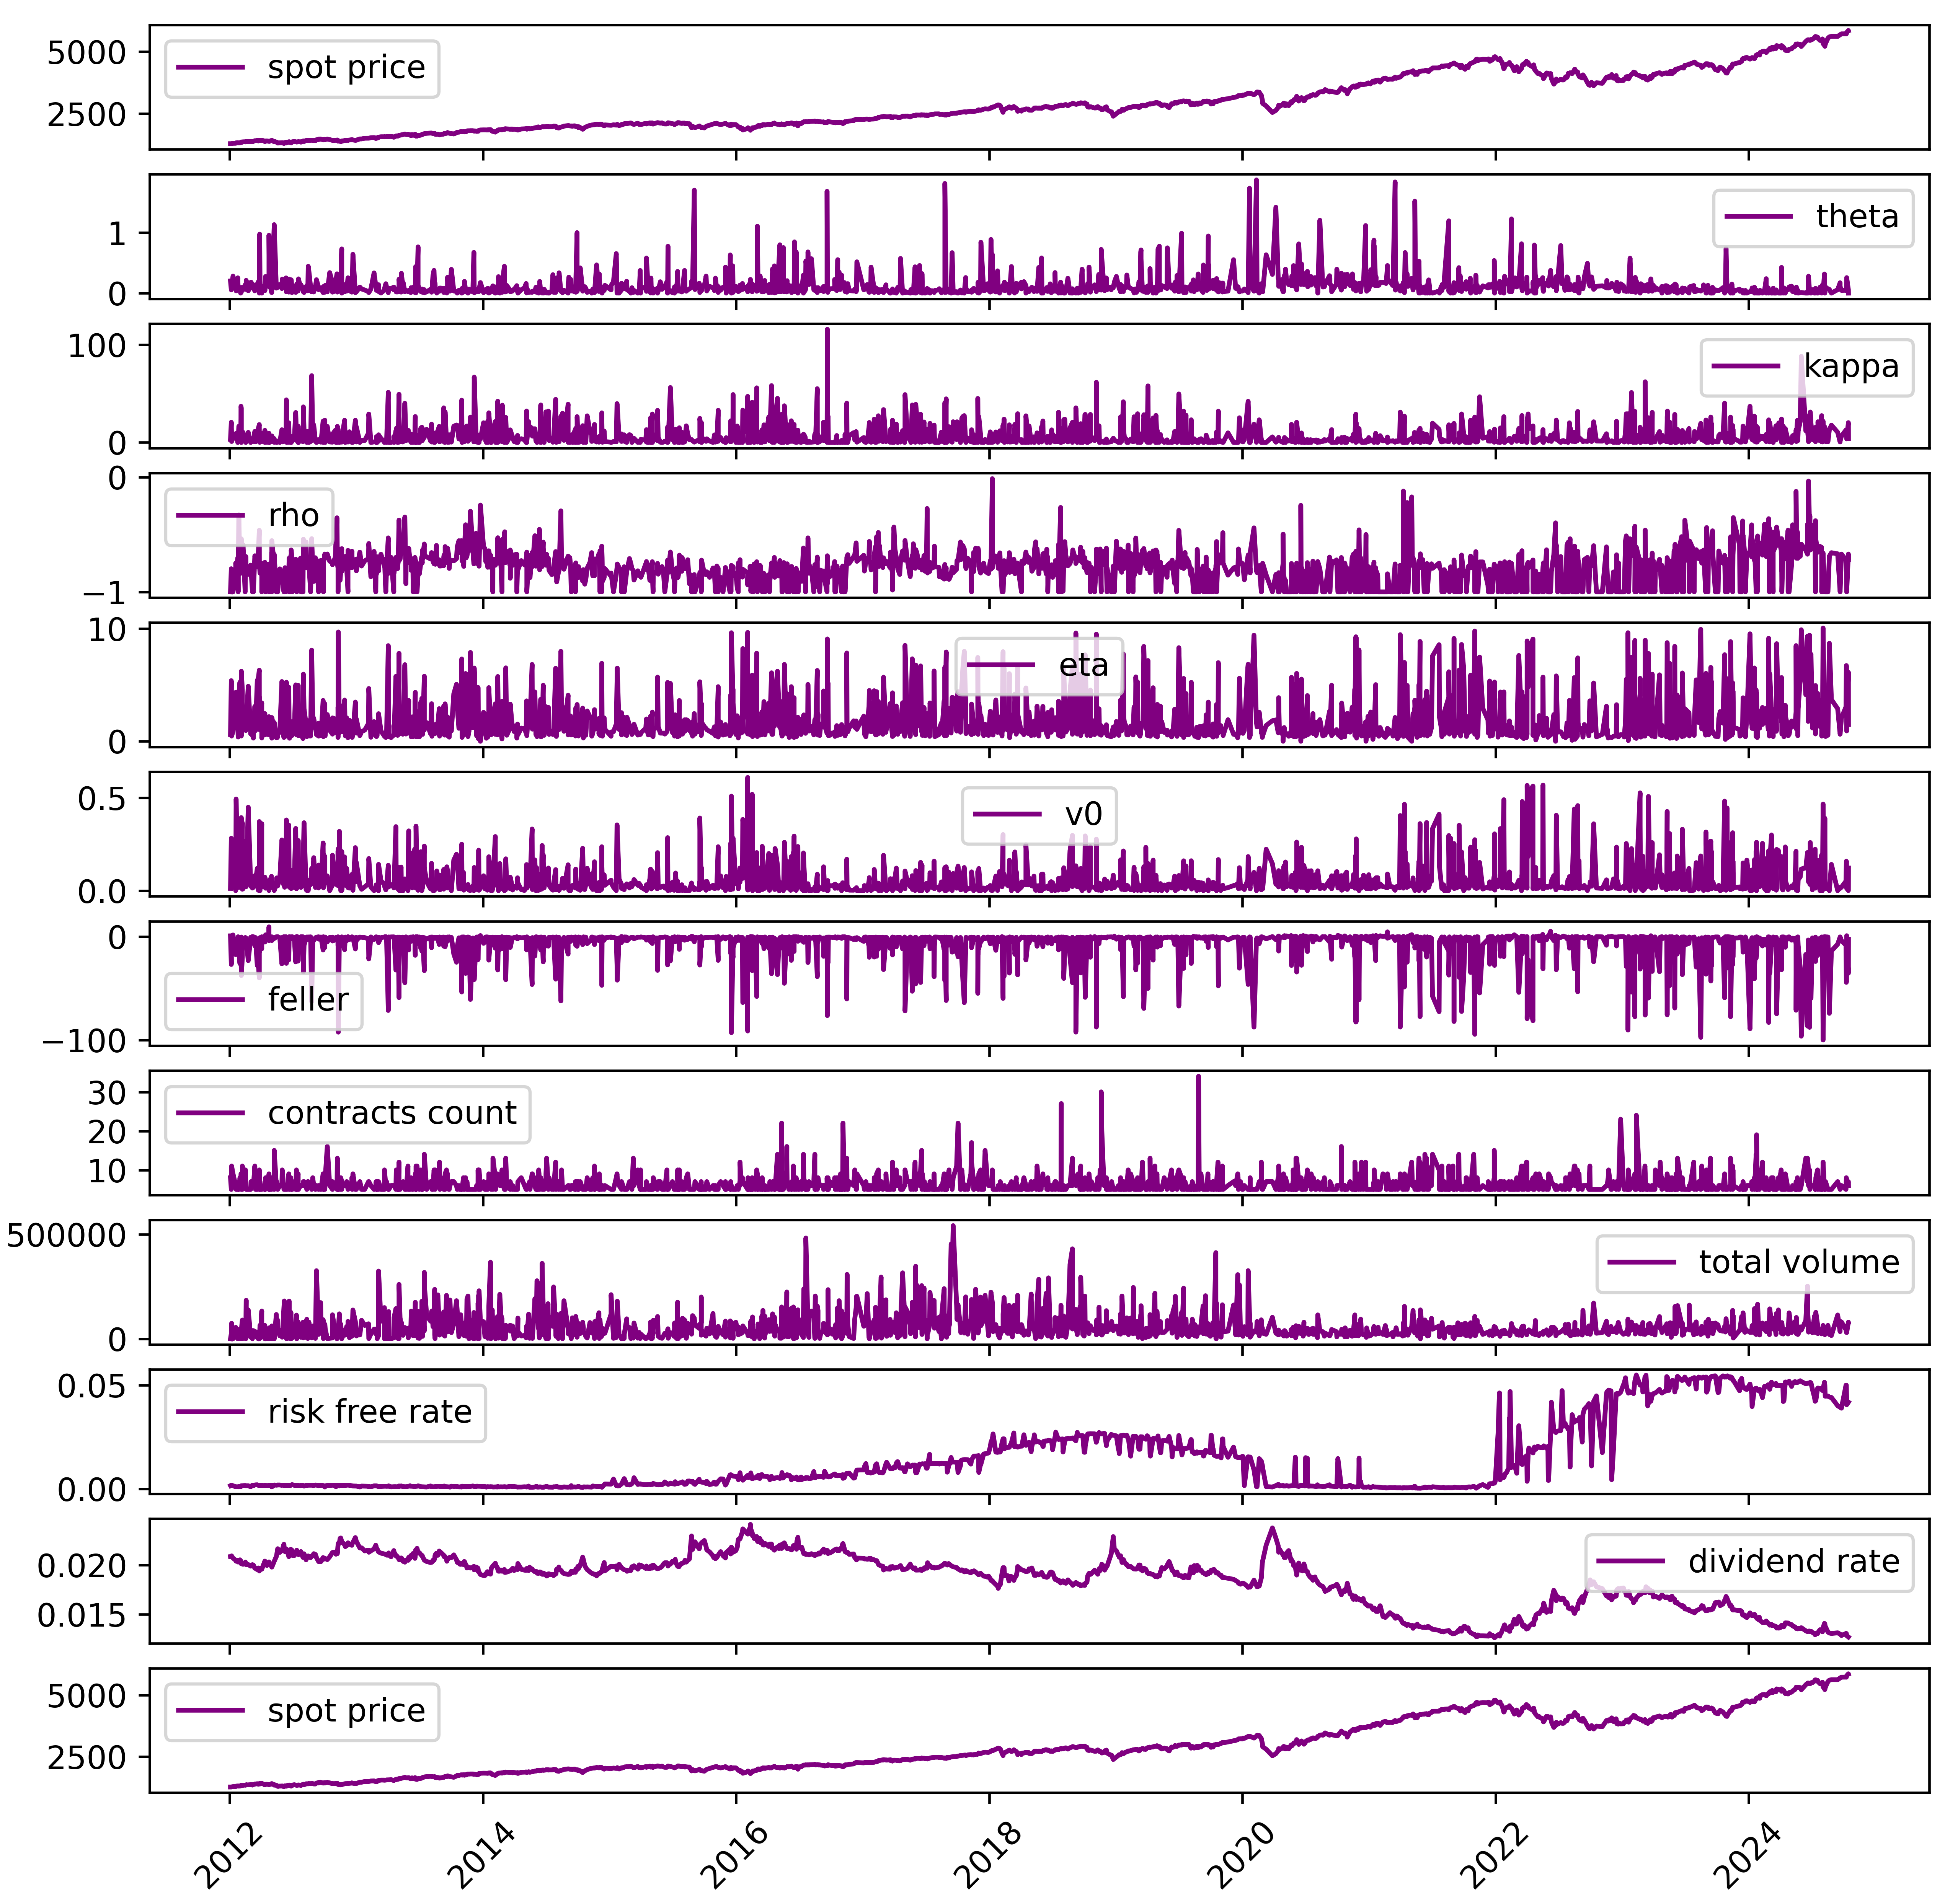
\includegraphics[width=0.8\textwidth]{calibrations.png}
				\caption{Plot of retrieved historical Heston \cite{heston_1993_a} model parameters, underlying $S$, risk-free, and dividend rates for the SPX options market}
				\label{fig:calibrations}
			\end{figure}
			\newpage
	
	\subsection{Barrier Option Price Functional}
		\vfill
		A Barrier option is a contingent claim on a financial security, in our case the plain European option, with the additional condition in the payoff function $C^{\text{payoff}} = (S_{T}-K)^{+}$ determining whether, at any point in the contract's tenor, the underlying spot price 'Knocks' 'In' or 'Out' (i.e., whether it breaks the barrier level):
		\vfill
		\begin{align}
			\begin{aligned}
				C^{\text{payoff}}_{\text{UpIn}} &= \mathbb{1}_{\{ S_t > B \,\forall\, t \}} \times (S_{T}-K)^{+}, \\
				C^{\text{payoff}}_{\text{UpOut}} &= \mathbb{1}_{\{ S_t < B \,\forall\, t \}} \times (S_{T}-K)^{+}, \\
				C^{\text{payoff}}_{\text{DownIn}} &= \mathbb{1}_{\{ S_t < B \,\forall\, t \}} \times (S_{T}-K)^{+}, \: \text{and} \\
				C^{\text{payoff}}_{\text{DownOut}} &= \mathbb{1}_{\{ S_t > B \,\forall\, t \}} \times (S_{T}-K)^{+}
			\end{aligned}
			\label{eq:BarrierPayoffs}
		\end{align}
		\vfill
		in the case of a European call option. Assuming we have the appropriate pricing function for one contract, we will then create a vectorized version $C^{\text{Barrier}}$ which can be defined as:
		\vfill
		\begin{align}
			C^{\text{Barrier}} = F_{t}(S_0, \kappa, \theta, \rho, \eta, v_{0}, r, g, K, B, R, D^{\text{call/put}}, D^{\text{DownIn/DownOut/UpIn/UpOut}}) \label{eq:Cbarrier}
		\end{align}
		\vfill
		Where the price of one Barrier option contract $C^{\text{Barrier}}$ is a function of
		\begin{enumerate}
			\item the underlying security price $S$~\eqref{eq:hdXt}, 
			\item the mean reversion speed $\kappa$ of the variance process to $\theta$~\eqref{eq:hdvt}, 
			\item the long-run mean of the variance process $\theta$~\eqref{eq:hdvt}, 
			\item the correlation $\rho$ between the variance process $v_t$ and the underlying price process $X_t$~\eqref{eq:hdXt}, 
			\item the volatility of the variance process $\eta$~\eqref{eq:hdvt}, 
			\item the initial volatility $v_{0}$~\eqref{eq:hdvt}, 
			\item the risk-free rate $r$, 
			\item the dividend rate $g$, 
			\item the strike price $K$, 
			\item the barrier level $B$, 
			\item the rebate $R$, 
			\item a logical operator $D^{\text{call/put}}$ to denote the underlying European option payoff function, and
			\item a logical operator $D^{\text{DownIn/DownOut/UpIn/UpOut}}$ denoting the barrier contract type~\eqref{eq:BarrierPayoffs},
		\end{enumerate}
		\vfill
		Barrier options are accurately priced using Monte Carlo simulation with control variates. However, to use this as a benchmark, we will first generate less accurate prices using a finite difference advection technique to save computational effort for our initial investigations into data generation, train set creation, and model testing.
		\vfill
		
	\newpage
	
	\subsection{Asian Option Price Functional}
		\vfill
		The Asian option is similarly a derivative of, in our case, a plain European option with payoff $(S_T-K)^{+}$ for call, and $(K-S_T)^{+}$ for put options. A supplementary condition is applied, defining the respective payoff functions as:
		\begin{align}
			C^{\text{Arithmetic}}_t &= e^{-r(T-t)} \times \frac{1}{m} \sum_{i=1}^{m} (S_{T}^{\text{Arithmetic}} - K)^{+} \\
			C^{\text{Geometric}}_t &= e^{-r(T-t)} \times \frac{1}{m} \sum_{i=1}^{m} (S_{T}^{\text{Geometric}} - K)^{+}
		\end{align} \label{eq:AsianPayoffs}
		where $S_{T}^{\text{Arithmetic}}$ and $S_{T}^{\text{Geometric}}$ are the arithmetic and geometric mean of the underlying spot price measured over predetermined points in time (i.e., the 'fixing' dates). It is also possible to price an Asian option which has past fixings (i.e., is not a fresh contract), However, for the purposes of this paper, we will only be considering Asian options at inception.
		\begin{align}
			S^{\text{Arithmetic}}_T = \frac{1}{n} \sum_{i=1}^{n} S^{i}_{t}, \hspace{1em} n \in \mathbb{N}, \; t_n = T
		\end{align} \label{eq:arithmeticavg}
		\begin{align}
			S^{\text{Geometric}}_T =  \sqrt[n]{\prod_{i=1}^{n} S^{i}_{t}}, \hspace{1em} n \in \mathbb{N}, \; t_n = T
		\end{align} \label{eq:geometricavg}
		\par
		Consequently, the vectorized Asian option pricing function can be defined as:
		\begin{align}
			C^{\text{Asian}} = F_{t}(S_0, \kappa, \theta, \rho, \eta, v_{0}, r, g, K, n, P, D^{\text{call/put}}, D^{\text{Arithmetic/Geometric}}) \label{eq:Casian}
		\end{align}
		where the price of an Asian option is a function of:
		\begin{enumerate}
			\item the underlying security price $S$~\eqref{eq:hdXt}, 
			\item the mean reversion speed $\kappa$ of the variance process to $\theta$~\eqref{eq:hdvt}, 
			\item the long-run mean of the variance process $\theta$~\eqref{eq:hdvt}, 
			\item the correlation $\rho$ between the variance process $v_t$ and the underlying price process $X_t$~\eqref{eq:hdXt}, 
			\item the volatility of the variance process $\eta$~\eqref{eq:hdvt}, 
			\item the initial volatility $v_{0}$~\eqref{eq:hdvt}, 
			\item the risk-free rate $r$, 
			\item the dividend rate $g$, 
			\item the strike price $K$, 
			\item the number of fixing dates $n$, 
			\item the number of past fixings$P$ which for our current purposes is always equal to zero, 
			\item a logical operator $D^{\text{call/put}}$ to denote the underlying European option payoff function, and
			\item a logical operator $D^{\text{Arithmetic/Geometric}}$ denoting the averaging type~\eqref{eq:AsianPayoffs},
		\end{enumerate}

	\vfill
	\newpage
	\vfill

\section{Data Generation Method}
	\label{sections:DataGenMeth}
	The proposed method for amplifying a matrix of variables into a higher dimensional space is to iterate through every row $i$ of the matrix, for each one generating a subset $X_{t}$ of the final feature matrix $X$.
	Suppose we consider a set of variables:
	\begin{align}
		\D = & 
		\begin{bmatrix}
			\D_{1,
				1} & \cdots & \D_{1,j} & \cdots & \D_{1,m} \\
			\vdots  & \ddots & \vdots & \reflectbox{$\ddots$} & \vdots  \\
			\D_{t,1} & \cdots & \D_{t,j} & \cdots & \D_{t,m}\\
			\vdots  & \reflectbox{$\ddots$} & \vdots & \ddots & \vdots \\
			\D_{n,1} & \cdots & \D_{n,j} & \cdots & \D_{n,m}
		\end{bmatrix} \label{eq:D}
	\end{align}
	We will amplify the initial feature matrix $\D$ by iterating along the row dimension, for each iteration constructing a set of vectors $H_{t}$ representing the possible values of all features individually:
	\begin{align}
		H_{t} = \{ \left[\D_{t,1}\right], \ldots, \left[\D_{t,j}\right], \ldots, \left[\D_{t,m}\right], F^{(1)}_{\D_{t}}, \ldots F^{(j)}_{\D_{t}}, \ldots, F^{(\tilde{m})}_{\D_{t}} \} \label{eq:Ht}
	\end{align}
	where each $F^{(j)}$ is a vector of chosen, possible auxiliary feature values which are dependent on the state of $\D_{t}$ for every observation $i$ and can also be a function of any feature $j$ in $\D_{t}$. This allows us to combine vectors of varying lengths and consistently obtain all combinations of their values. The feature matrix $X_{t}$ can then be defined as the Cartesian product of all elements in $H_{t}$:
	\begin{equation}
		\begin{aligned}
			X_{t} = \{ (H_{t}^{(1)}, \ldots, H_{t}^{(j)}, \ldots, H_{t}^{(k)}) \mid H_{t}^{(1)} \in H_{t}^{(1)}, \ldots, H_{t}^{(j)} \in H_{t}^{(j)}, \ldots, H_{t}^{(k)} \in H_{t}^{(k)} \} \label{eq:Xt}
		\end{aligned}
	\end{equation}
	where $X_{t}$ has dimension $(k \times s)$. Naturally occurring identities of this construction are that $k = m + \tilde{m}$ and $s = \prod_{j=1}^k \dim(H_{t}^{(j)})$.
	The creation of one feature matrix $X_{t}$ is, in essence, a simulation of the specified system for one observation of possible and feasible feature states in $t$. The combination of all $X_{t}$ for $n$ observations of the system's condition at every $t$ will result in the final feature matrix $X$ which we will be using for the models' initial development according to the specifications in~\ref{sections:HDt} and~\ref{sections:contractMethods}.
	
\section{Application of data generation method~\ref{sections:DataGenMeth} to path-dependent index options}
	\label{sections:specrationale}
	In the spirit of Liu et. al. \cite{liu_2019_pricing} and Frey et. al. \cite{frey_2022_option} we will generate a development dataset by simulating possible parameter combinations for a given security. Liu et. al. \cite{liu_2019_pricing} demonstrate a considerable increase in computational efficiency with retention of low errors for the estimation of implied volatilities via artificial neural networks by considering the relative spot price (i.e., the spot price $S$ divided by the strike price $K$) and the relative option price (i.e., the option's price $C$ divided by its strike $K$) as opposed to their levels, a method we will be borrowing for our estimation. Frey et. al. \cite{frey_2022_option} propose a data generation method via Cartesian product to create a multi-dimensional sample space representing an option's price as a functional form of its features. We therefore propose the augmented data generation method \ref{sections:DataGenMeth} utilizing Cartesian product to generate path-dependent contract features while considering the option's relative price ($C/K$) and any other linear features also scaled by the strike price $K$.
	\par
	It can be said in more general terms, that we will collect a matrix $\D$~\eqref{eq:D} representing market conditions to be augmented with auxiliary variables $F^{(j)}_{\D_{t}}$~\eqref{eq:Ht}, in essence simulating all but strictly pheasible contract combinations. We augment this sample space to cover all possible feature values of interest against which we train a neural network to obtain a highly efficient numerical approximation of the pricing function used to generate our target variable.
	
	\subsection{Defining the market condition parameter matrix $\D$~\eqref{eq:D}}
	\label{sections:HDt}
	Following the collection of $n$ Heston \cite{heston_1993_a} model parameter observations in time $i$, we are able to define the initial feature matrix $\D$~\eqref{eq:D} as:
	\begin{align}
		\D^{\text{Heston}} = &
		\begin{bmatrix} 
			S_{1} & \kappa_1 & \theta_1 & \rho_1 & \eta_1 & v_{1} & r_1 & g_1 \\
			\vdots & \vdots & \vdots & \vdots & \vdots & \vdots & \vdots & \vdots \\
			S_{t} & \kappa_{t} & \theta_{t} & \rho_{t} & \eta_{t} & v_{t} & r_{t} & g_{t} \\
			\vdots & \vdots & \vdots & \vdots & \vdots & \vdots & \vdots & \vdots \\
			S_{n} & \kappa_n & \theta_n & \rho_n & \eta_n & v_{n} & r_n & g_n \\
		\end{bmatrix} \label{eq:HD}
	\end{align}
	consisting of $n$ historically observed sets of Heston \cite{heston_1993_a} parameters as in \eqref{eq:hdXt} and \eqref{eq:hdvt}, underlying spot prices $S$, risk-free rates $r$, and dividend rates $g$ where $S$ and $v_0$ are represented as $S$ and $v$ respectively to simplify notation. An approach drawing from Liu. et. al. \cite{liu_2019_pricing}.
	\subsection{Contract Specific Methods}
		\label{sections:contractMethods}
		\subsubsection{Constructing $X^{\text{Barrier}}$}
			In order to simulate the multidimensional space representing a Barrier option's price as a function of its features, we begin by iterating through the row dimension of $\D^{\text{Heston}}$~\eqref{eq:HD}, for each row constructing a set $H_{t}$~\eqref{eq:Ht} with auxiliary variables $F_{\D_{t}}^{(j)}$ defined as:
			\begin{equation}
				\begin{aligned}
					F_{\D_{t}}^{(1)} &= K_{S} = \left[ k_1, \ldots, k_j, \ldots, k_h \right], \quad  k_1 < S < k_h, \quad k_{\tilde{j}} < k_j \, \forall \, \tilde{j} < j, \\
					F_{\D_{t}}^{(2)} &= T = \left[ \tau_1, \ldots, \tau_{t}, \ldots, \tau_h \right], \\
					F_{\D_{t}}^{(3)} &= B = \left[ B_1, \ldots, B_j, \ldots, B_h \right], \quad  B_1 < S < B_h, \quad B_{\tilde{j}} < B_j \, \forall \, \tilde{j} < j, \\
					F_{\D_{t}}^{(4)} &= R = \left[0\right], \\
					F_{\D_{t}}^{(5)} &= F^{\text{call/put}} = \left[ D^{\text{call}}, D^{\text{put}} \right], \\
					F_{\D_{t}}^{(6)} &= F^{\text{Out/In}} = \left[D^{\text{Out}}, D^{\text{In}}\right],
				\end{aligned}
			\end{equation}
			where
			\begin{enumerate}
				\item $K_{S}$ is a set of strikes spread around the spot,
				\item $T$ is a set of maturities,
				\item $B$ is a set of barrier levels,
				\item $R$ is a set of rebates, which for the purposes of this study is a set consisting of only the element $0$ (zero),
				\item $F^{\text{call/put}}$ is a set of categorical variables representing the type of underlying European option, and
				\item $F^{\text{Out/In}}$ is a set of categorical variables representing the Barrier option type payoff.
			\end{enumerate}
			It is to be noted that the only feasible combinations are 'Down' options with $B<S$ and 'Up' with $B>S$ where $B$ is the Barrier level and $S$ is the underlying $S_{t}$ at time $i$.
			The subset feature matrix $X^{\text{Barrier}}_{t}$ will subsequently be defined as:
			\begin{align}
				X^{\text{Barrier}}_{t} &= 
				\scalebox{0.8}{$
					\left[
					\begin{array}{cccccccccccccc}
						S_{t} & \kappa_{t} & \theta_{t} & \rho_{t} & \eta_{t} & v_{t} & r_{t} & g_{t} & k_{1} &\tau_{1} & b_{1} & r^{\text{rebate}}_{1} & D^{\text{call/put}}_{1} & D^{\text{barrier type}}_{1} \\
						\vdots & \vdots & \vdots & \vdots & \vdots & \vdots & \vdots & \vdots & \vdots & \vdots & \vdots & \vdots & \vdots & \vdots \\
						S_{t} & \kappa_{t} & \theta_{t} & \rho_{t} & \eta_{t} & v_{t} & r_{t} & g_{t} & k_{s} & t_{s} & n_{s} & r^{\text{rebate}}_{s} & D^{\text{call/put}}_{s} & D^{\text{barrier type}}_{s} \\
					\end{array}
					\right]$} \label{eq:BXt}
			\end{align}
			essentially allowing us to generate $k$ contracts at every observation across the rows (discrete observations in time) of our initial feature matrix $\D^{\text{Heston}}$~\eqref{eq:HD} where the features carried over into $H_{t}$~\eqref{eq:Ht} from $\D_{t}$~\eqref{eq:D} are constant.
		
		\subsubsection{Constructing $X^{\text{Asian}}$}
			\vfill
			In the case of Asian options, the feature matrix generation process is not as straight forward. In order to simulate an evenly distributed sample space, we need to take into account the relationship between an Asian option's maturity and its fixing dates. This will require careful construction of a maturities vector $T$, ensuring the congruency of feature combinations. Therefore, we must consider a set of maturities defined as
			\begin{align}
				T^{\text{Asian}} = \left[ \tau_1, \ldots, \tau_{i}, \ldots, \tau_{h} \right] \label{eq:asianmats}
			\end{align}
			which will proceed the creation of $\dim{(T)}$ subsets within $X_{t}$\eqref{eq:Xt}. Subsequently, every subset is generated by considering the $H^{(i)}_{t}$~\eqref{eq:Ht} feature set with auxiliary variables $F_{\D_{t}}^{(j)}$ defined as:
			\begin{equation}
				\begin{aligned}
					F_{\D_{t}}^{(1)} &= T = \left[ \tau_{i} \right], \\
					F_{\D_{t}}^{(2)} &= K_{S} = \left[ k_1, \ldots, k_{i}, \ldots, k_{h} \right], \quad  k_1 < S < k_t, \quad k_{\tilde{j}} < k_j \, \forall \, \tilde{j} < j, \\
					F_{\D_{t}}^{(3)} &= A_{\tau} = \left[ a_1, \ldots, a_{i}, \ldots, a_{h} \right], \quad a_{h} \leq \tau \, \forall \, i, \\
					F_{\D_{t}}^{(4)} &= P = \left[ 0 \right], \\
					F_{\D_{t}}^{(5)} &= F^{\text{call/put}} = \left[ D^{\text{call}}, D^{\text{put}} \right], \\
					F_{\D_{t}}^{(6)} &= F^{\text{arithmetic/geometric}} = \left[ D^{\text{arithmetic}}, D^{\text{geometric}} \right].
				\end{aligned}
			\end{equation}
			where
			\begin{enumerate}
				\item $\tau$ is the iterated maturity in $T^{\text{Asian}}$~\eqref{eq:asianmats},
				\item $K_{S}$ is a set of strikes spread around the spot price $S$,
				\item $A_{\tau}$ are factors of $\tau$ which will determine the number of fixing dates applicable to the contract,
				\item $P$ is a set of past fixings, which for the purposes of this study is a set consisting of only the element $0$ (zero),
				\item $F^{\text{call/put}}$ is a set of categorical variables representing the type of underlying European option, and
				\item $F^{\text{arithmetic/geometric}}$ is a set of categorical variables representing the contract's averaging type.
			\end{enumerate}
			\vfill
			The subset feature matrix $X^{\text{Asian}}_{t}$ will subsequently be defined as:
			\begin{align}
				X^{\text{Asian}}_{t} &= 
				\scalebox{0.8}{$
					\left[
					\begin{array}{cccccccccccccc}
						S_{t} & \kappa_{t} & \theta_{t} & \rho_{t} & \eta_{t} & v_{t} & r_{t} & g_{t} & k_{1} & \tau_{1} & a_{1} & p_{1} & D^{\text{call/put}}_{1} & D^{\text{arithmetic/geometric}}_{1} \\
						\vdots & \vdots & \vdots & \vdots & \vdots & \vdots & \vdots & \vdots & \vdots & \vdots & \vdots & \vdots & \vdots & \vdots \\
						S_{t} & \kappa_{t} & \theta_{t} & \rho_{t} & \eta_{t} & v_{t} & r_{t} & g_{t} & k_{s} & \tau_{s} & a_{s} & p_{s} & D^{\text{call/put}}_{s} & D^{\text{arithmetic/geometric}}_{s} \\
					\end{array}
					\right]$} \label{eq:AXt}
			\end{align}
			essentially allowing us to generate $s$ contracts at every observation across the rows (discrete observations in time) of our initial feature matrix $\D^{\text{Heston}}$~\eqref{eq:HD} where the features carried over into $H_{t}$~\eqref{eq:Ht} from $\D_{t}$~\eqref{eq:D} are constant.
		
	\vfill
	\newpage

\section{Model Training}
	With adequate data, we may begin training our multi-layer perceptron network to numerically approximate the relationship between our feature matrix $X$ and target vector $y$.
	\par
	\begin{figure}[h]
		\centering
		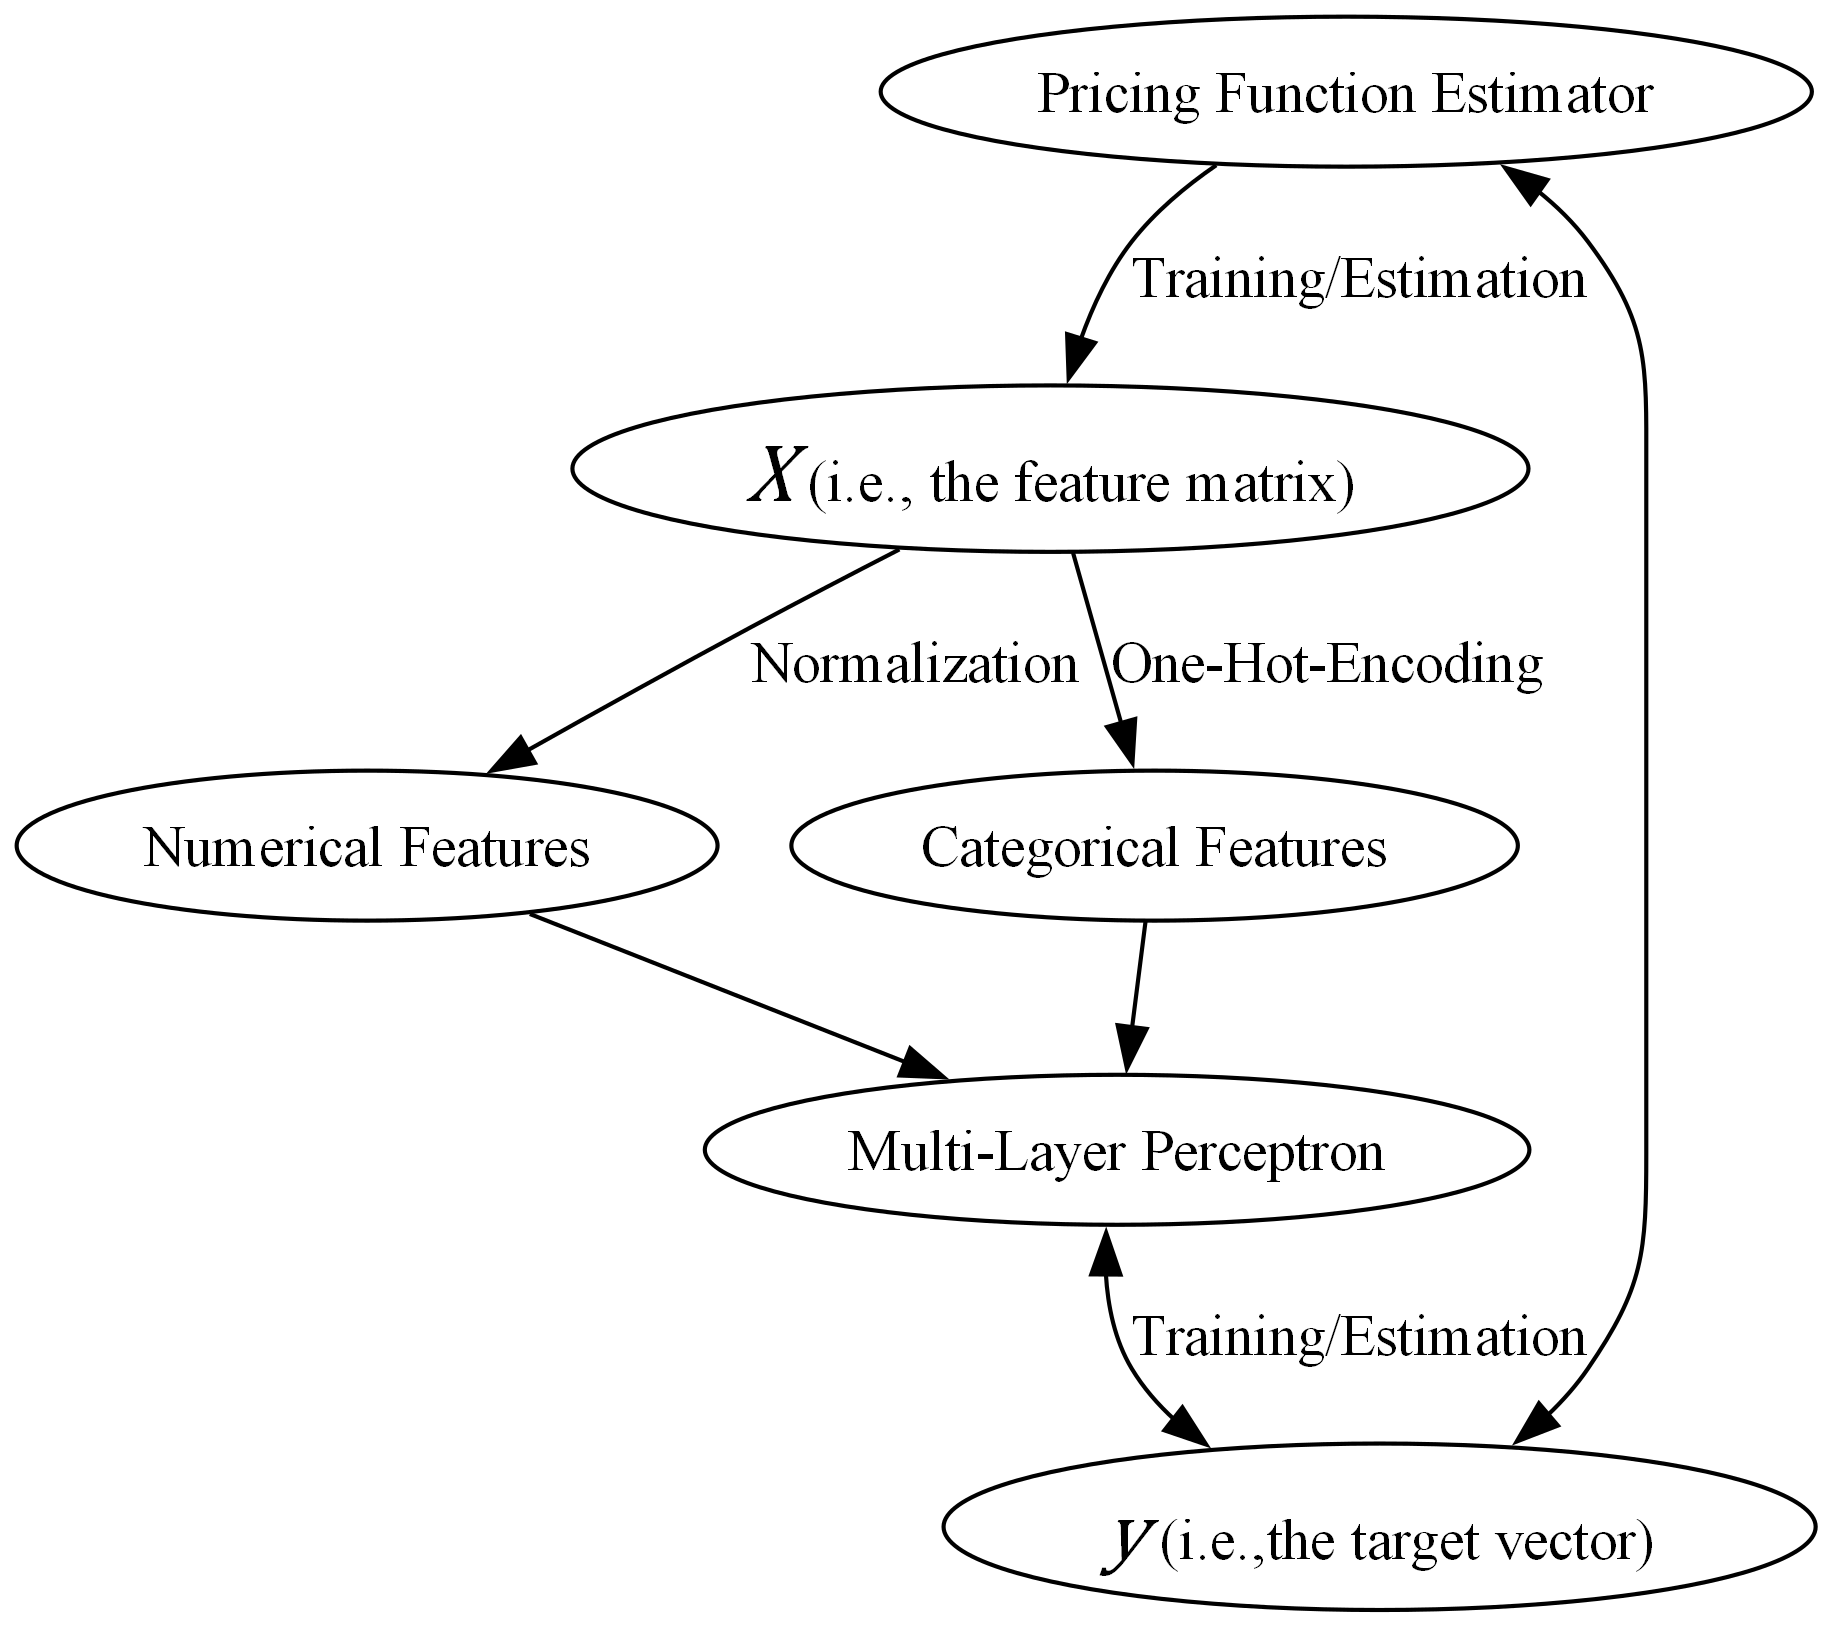
\includegraphics[width=0.7\textwidth]{MLP.png}
		\caption{Graph of multi-layer perceptron Pricing Estimator}
		\label{fig:MLP}
	\end{figure}
	\subsection{Multi-layer perceptron Specification}
		Technically, the neural network itself is a directed acyclic graph whose architecture and parametrization varies depending on the data being estimated. A general representation of a three-layer neural network with $h$ total neurons in its 'hidden' layer can be depicted as \\
%		\begin{figure}[h]
%			\centering
%			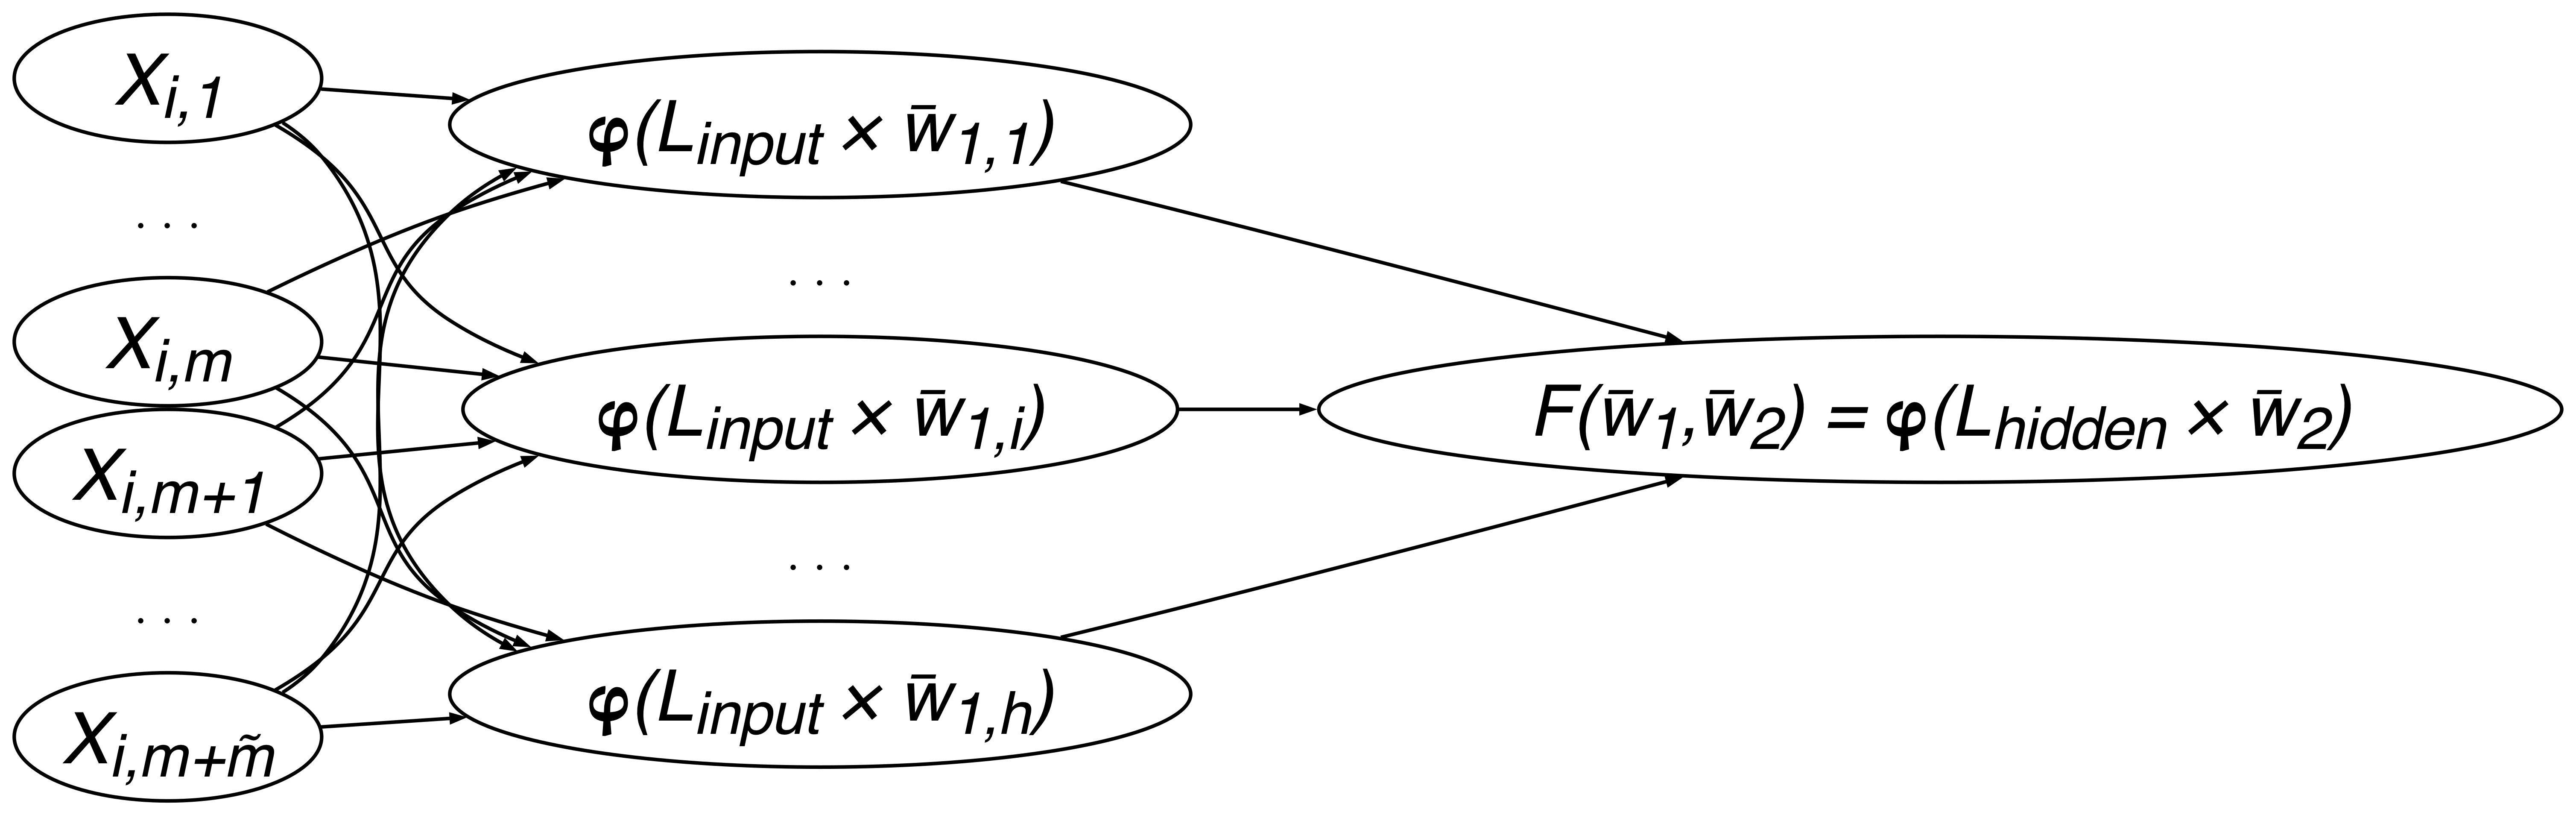
\includegraphics[width=0.8\textwidth]{elip.png}
%		\end{figure}
		\resizebox{\textwidth}{!}{%
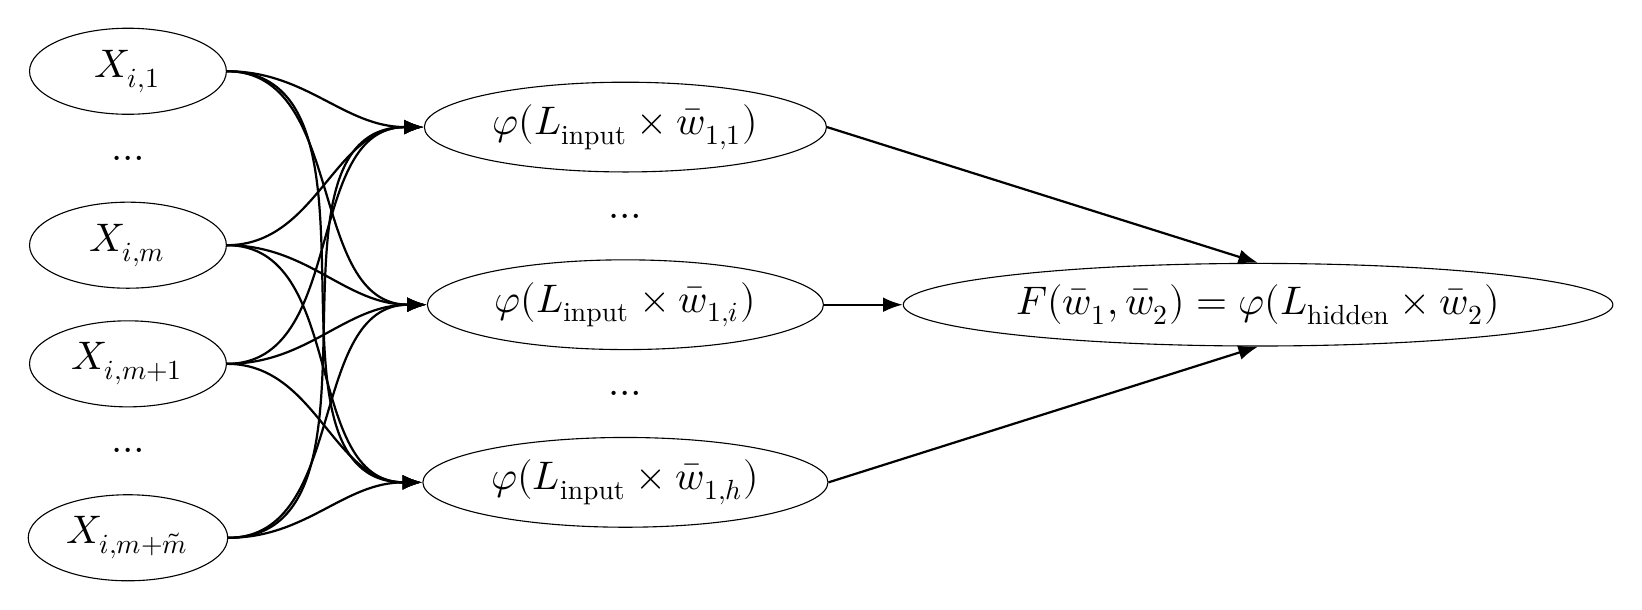
\begin{tikzpicture}[
	every node/.style={font=\Large},
	input/.style={draw, ellipse, minimum width=2.2cm, align=center},
	hidden/.style={draw, ellipse, minimum width=4.5cm, align=center},
	output/.style={draw, ellipse, minimum width=7.5cm, align=center},
	arrow/.style={-{Latex[length=2.5mm]}, thick}
	]
	
	% Input layer (spread vertically)
	\node[input,ellipse,minimum width=2.5cm] (x1) {$X_{i,1}$};
	\node (dots1) [below=0.4cm of x1] {$\hdots$};
	\node[input,ellipse,minimum width=2.5cm] (xm) [below=0.4cm of dots1] {$X_{i,m}$};
	\node[input,ellipse,minimum width=2.5cm] (x1p) [below=0.4cm of xm] {$X_{i,m+1}$};
	\node (dots2) [below=0.4cm of x1p] {$\hdots$};
	\node[input,ellipse,minimum width=2.5cm] (xt) [below=0.4cm of dots2] {$X_{i,m+\tilde{m}}$};
	
	% Hidden layer (centered horizontally and vertically)
	\node[hidden, right=2.5cm of xm, yshift=1.5cm] (h1) {$\varphi(L_{\text{input}} \times \bar{w}_{1,1})$};
	\node (hdots1) [below=0.4cm of h1] {$\hdots$};
	\node[hidden, below=0.4cm of hdots1] (hi) {$\varphi(L_{\text{input}} \times \bar{w}_{1,i})$};
	\node (hdots2) [below=0.4cm of hi] {$\hdots$};
	\node[hidden, below=0.4cm of hdots2] (hh) {$\varphi(L_{\text{input}} \times \bar{w}_{1,h})$};
	
	% Output layer (centered vertically relative to hidden layer)
	\node[output, right=1cm of hi] (out) 
	{$F(\bar{w}_{1},\bar{w}_{2}) = \varphi(L_{\text{hidden}} \times \bar{w}_{2})$};
	
	% Connections (curved)
	\foreach \i in {x1, xm, x1p, xt} {
		\draw[arrow] (\i.east) to[out=0,in=180] (h1.west);
		\draw[arrow] (\i.east) to[out=0,in=180] (hi.west);
		\draw[arrow] (\i.east) to[out=0,in=180] (hh.west);
	}
	
	\draw[arrow] (h1.east) -- (out.north);
	\draw[arrow] (hi.east) -- (out.west);
	\draw[arrow] (hh.east) -- (out.south);
	
\end{tikzpicture}
}
		\noindent
		where $\varphi$ is the activation function ReLU, $L_{\text{input}}$ is the vector of normalized input features, and $L_{\text{hidden}}$ is the vector of node values weighted by the hidden layer. Solving the model involves minimization of a loss function, in our case the squared error between the estimated $\hat{y}_{i}$ and the target $y_{i}$ for all $N = n \times s$ observations in our feature matrix $X$:
		\begin{equation}
			\min_{w_{1}, w_{2}} \, \frac{1}{N} \sum_{i=1}^{N} \left(F_{t}(w_{1}, w_{2}) - y_{t}\right)^{2}
		\end{equation}
		\par
		We begin constructing the neural network as depicted in figure~\ref{fig:MLP}, choosing appropriate inputs and general architecture given our intentions and mathematical intuition. However, to obtain at least quasi-pertinent results, one needs to establish reasonable solving parameters.
		\vspace{0.5em}
	
		\begin{minipage}{0.45\textwidth}
	\subsection{Asian Option Network}
	\label{sections:AsianNet}
	\centering
	\begin{tabular}{ll}
		\toprule
		feature & transformation \\
		\midrule
		days\_to\_maturity & StandardScaler \\
		fixing\_frequency & StandardScaler \\
		past\_fixings & StandardScaler \\
		risk\_free\_rate & StandardScaler \\
		dividend\_rate & StandardScaler \\
		kappa & StandardScaler \\
		theta & StandardScaler \\
		rho & StandardScaler \\
		eta & StandardScaler \\
		v0 & StandardScaler \\
		relative\_spot & StandardScaler \\
		averaging\_type & OneHotEncoder \\
		w & OneHotEncoder \\
		\bottomrule
	\end{tabular}
	
	\vspace{0.5em}
	\begin{tabular}{ll}
		\toprule
		parameter & specification \\
		\midrule
		activation & relu \\
		solver & sgd \\
		alpha & 0.0001 \\
		batch_size & auto \\
		learning_rate & adaptive \\
		learning_rate_{t}nit & 0.1 \\
		power_t & 0.5 \\
		max_{t}ter & 500 \\
		loss & squared_error \\
		hidden_layer_sizes & (20,) \\
		shuffle & True \\
		random_state & 710 \\
		tol & 0.0001 \\
		verbose & False \\
		warm_start & False \\
		momentum & 0.9 \\
		nesterovs_momentum & True \\
		early_stopping & True \\
		validation_fraction & 0.1 \\
		beta_1 & 0.9 \\
		beta_2 & 0.999 \\
		epsilon & 1e-08 \\
		n_{t}ter_no_change & 20 \\
		max_fun & 15000 \\
		\bottomrule
	\end{tabular}
\end{minipage}
\begin{minipage}{0.45\textwidth}
	\subsection{Barrier Option Network}
	\label{sections:barrierNet}
	\centering
	\begin{tabular}{ll}
		\toprule
		feature & transformation \\
		\midrule
		days_to_maturity & StandardScaler \\
		dividend_rate & StandardScaler \\
		risk_free_rate & StandardScaler \\
		theta & StandardScaler \\
		kappa & StandardScaler \\
		rho & StandardScaler \\
		eta & StandardScaler \\
		v0 & StandardScaler \\
		relative_spot & StandardScaler \\
		relative_barrier & StandardScaler \\
		relative_rebate & StandardScaler \\
		barrier_type_name & OneHotEncoder \\
		w & OneHotEncoder \\
		\bottomrule
	\end{tabular}
	\vspace{0.5em}
	
	\begin{tabular}{ll}
		\toprule
		parameter & specification \\
		\midrule
		activation & relu \\
		solver & sgd \\
		alpha & 0.0001 \\
		batch_size & auto \\
		learning_rate & adaptive \\
		learning_rate_{t}nit & 0.1 \\
		power_t & 0.5 \\
		max_{t}ter & 500 \\
		loss & squared_error \\
		hidden_layer_sizes & (10,) \\
		shuffle & True \\
		random_state & 710 \\
		tol & 0.0001 \\
		verbose & False \\
		warm_start & False \\
		momentum & 0.9 \\
		nesterovs_momentum & True \\
		early_stopping & True \\
		validation_fraction & 0.1 \\
		beta_1 & 0.9 \\
		beta_2 & 0.999 \\
		epsilon & 1e-08 \\
		n_{t}ter_no_change & 20 \\
		max_fun & 15000 \\
		\bottomrule
	\end{tabular}
\end{minipage}
		\par
		We achieve the above parametrizations after checking 6480 different parameter combinations determined by a grid of values we consider to be intuitively reasonable. While this method is severely computationally heavy, it allows both in-sample and out-of-sample errors to remain below five percent for Asian options, with in-sample error being usually around fifty basis points.
	
\section{Model Testing}
	\subsection{Model Performance}
	
		\begin{figure}[htbp]
			\centering
			\begin{minipage}{0.48\textwidth}
				\centering
				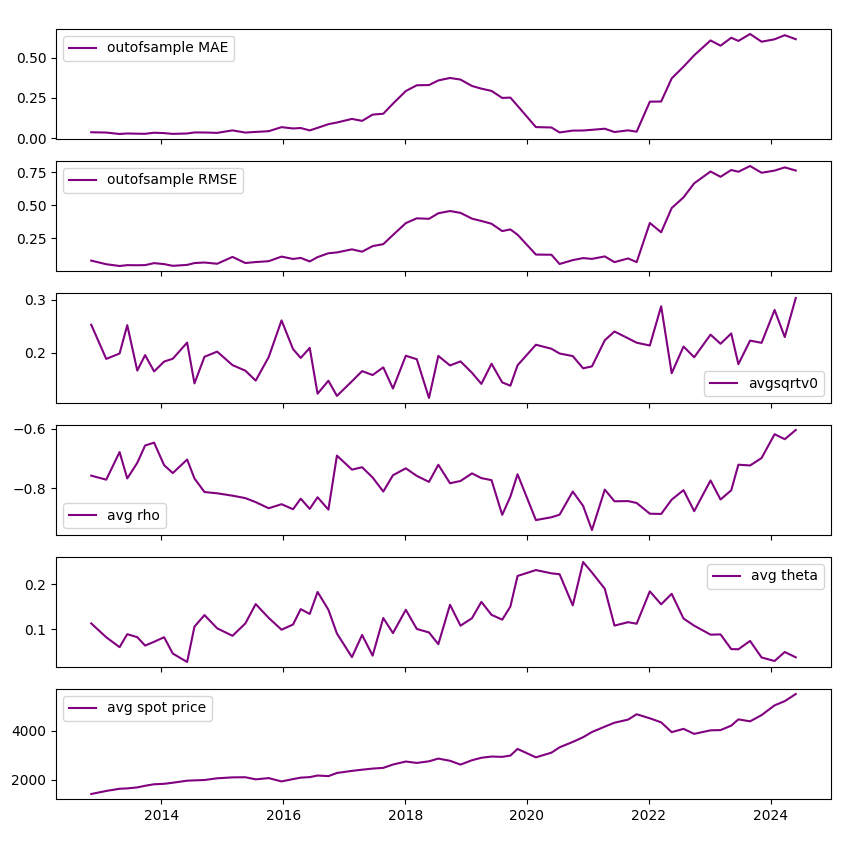
\includegraphics[width=\textwidth]{barrier errors.png}
				\caption{Out-of-sample average errors for barrier options}
				\label{fig:barrierErrors}
			\end{minipage}%
			\hfill
			\begin{minipage}{0.48\textwidth}
				\centering
				\includegraphics[width=\textwidth]{Asian errors.png}
				\caption{Out-of-sample average errors for Asian options}
				\label{fig:asianErrors}
			\end{minipage}
		\end{figure}%
		
		We notice that error increases without retraining of the model, likely due to it encountering previously unseen parameter value combinations.
		
	\subsection{Shapeliness of values}
		The neural network estimator can accurately produce the distribution of relative prices in the training set.
		\begin{figure}[htbp]
			\centering
			\begin{minipage}{0.48\textwidth}
				\centering
				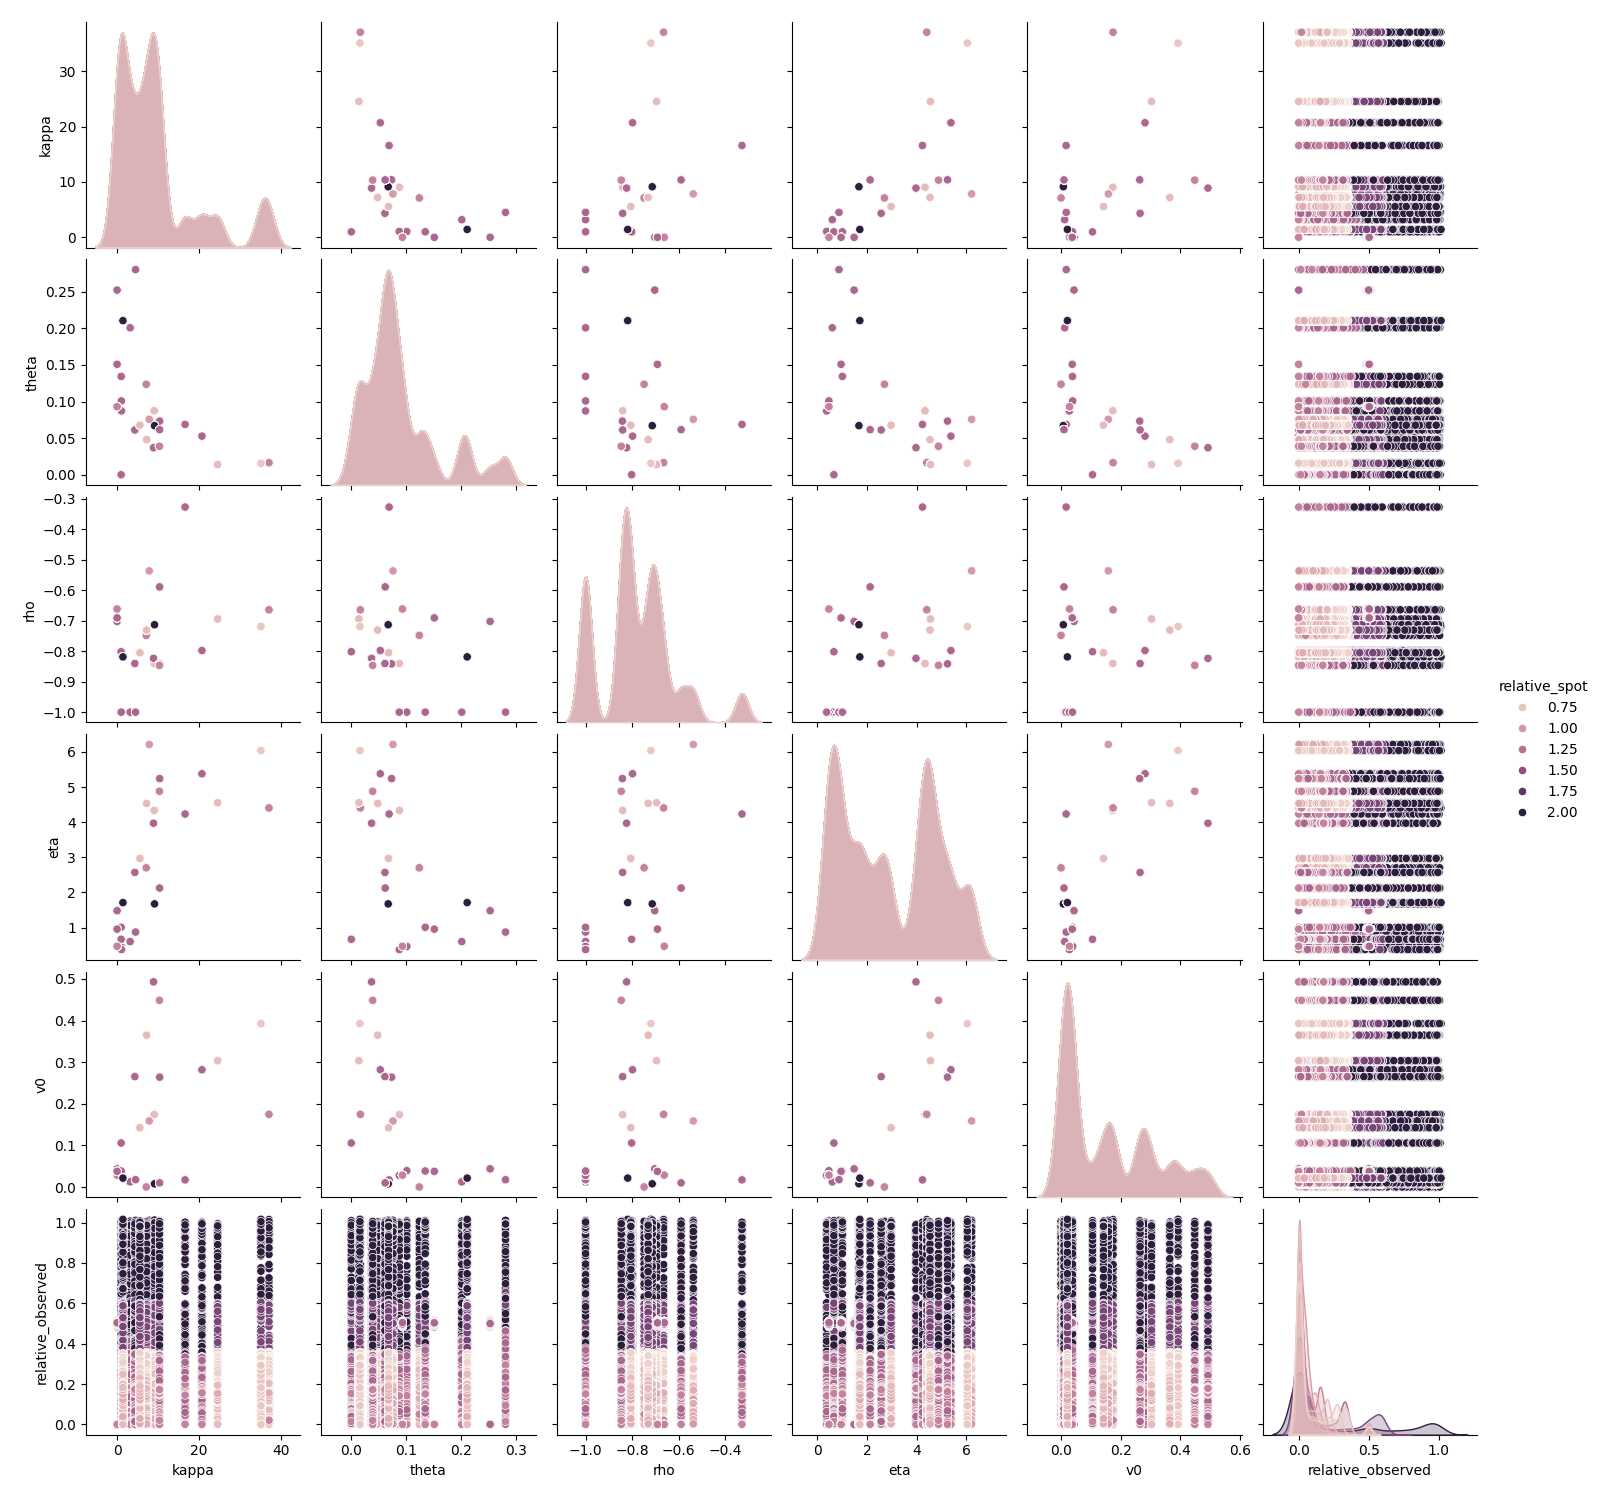
\includegraphics[width=\textwidth]{Shapely Barriers.png}
				\caption{Joint distribution of Barrier Option prices and Heston~\cite{heston_1993_a} model paramters}
				\label{fig:shapelyBarriers}
			\end{minipage}%
			\hfill
			\begin{minipage}{0.48\textwidth}
				\centering
				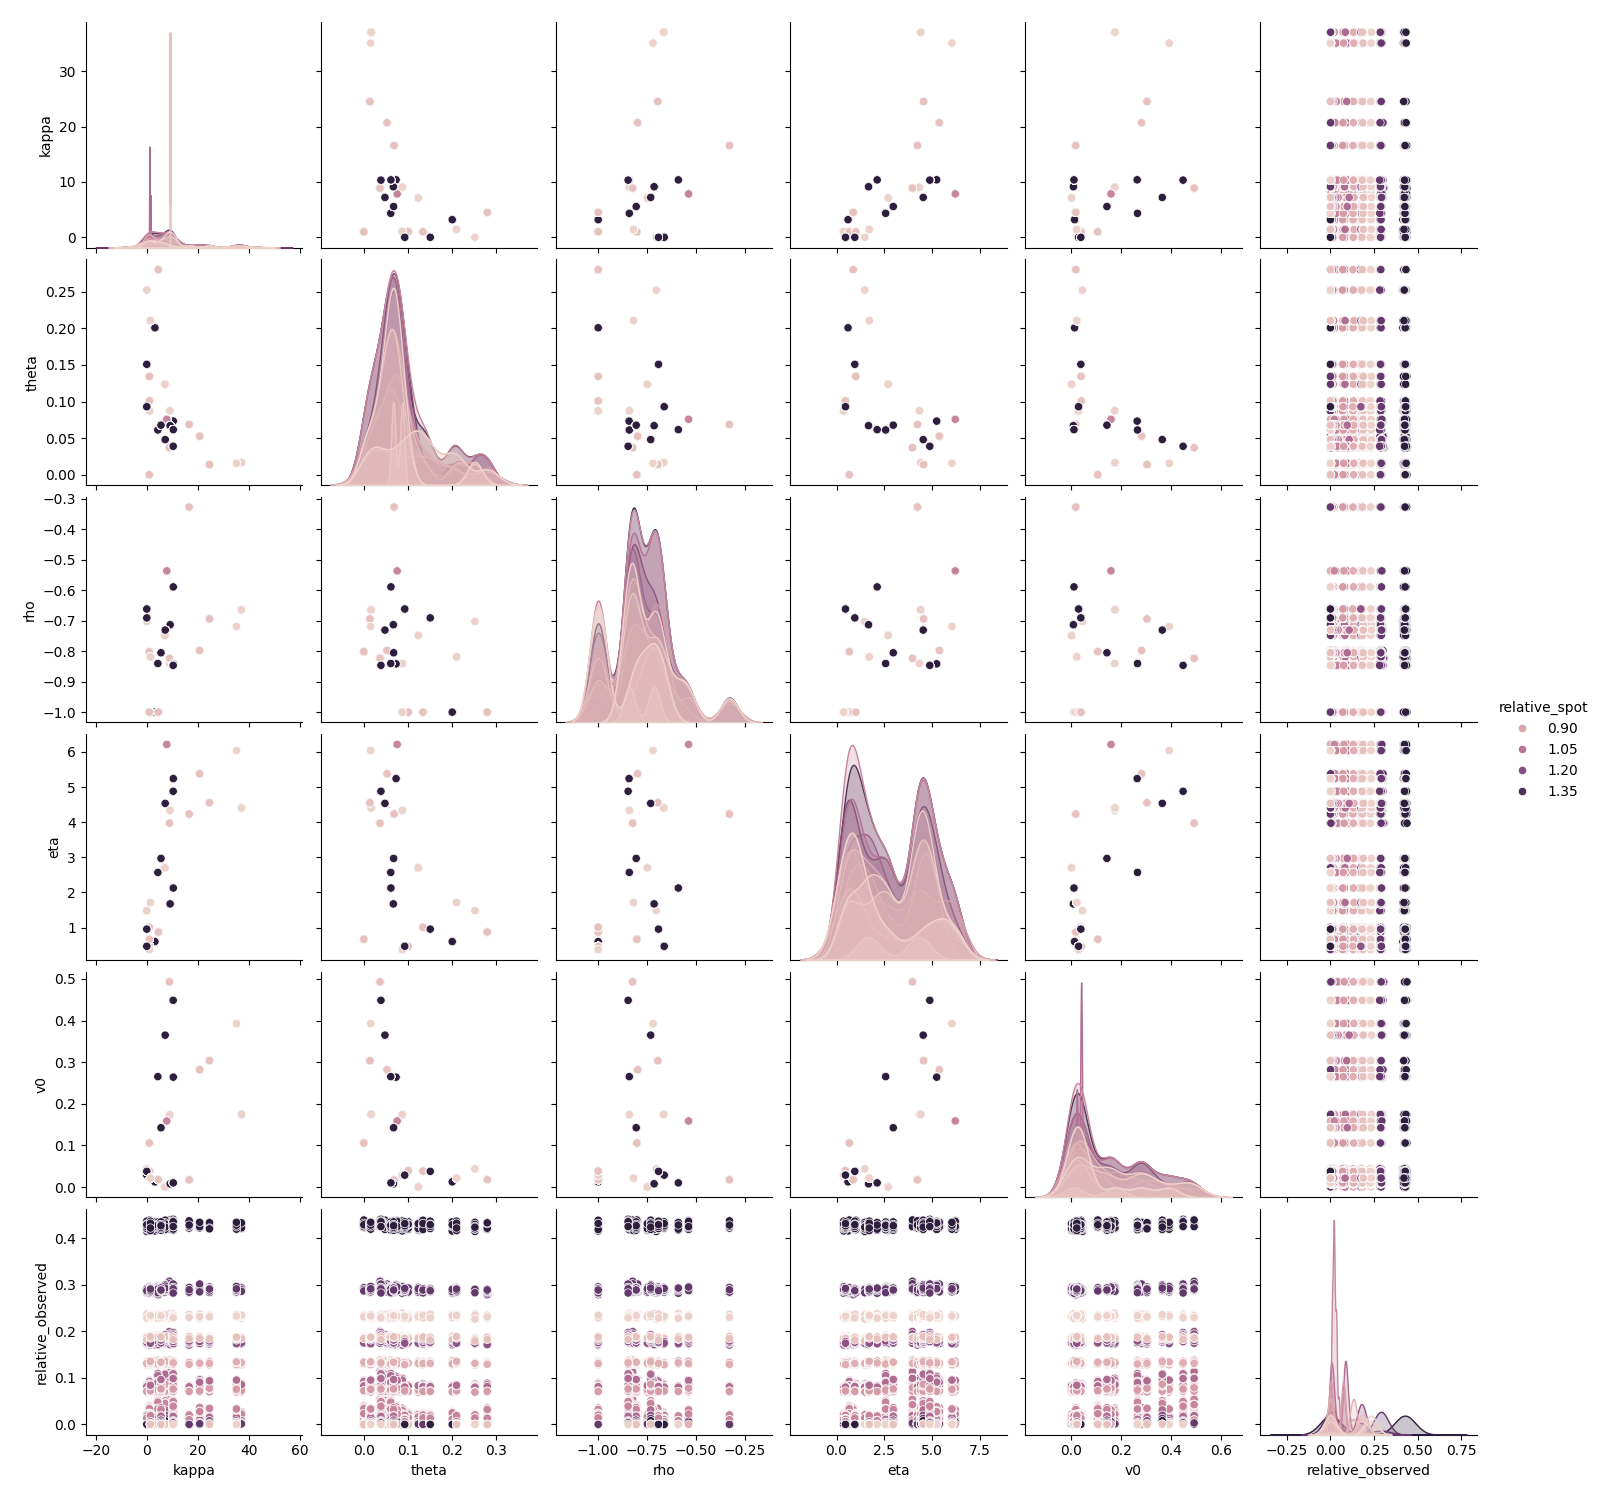
\includegraphics[width=\textwidth]{Shapely Asians.png}
				\caption{Joint distribution of Asian Option prices and Heston~\cite{heston_1993_a} model paramters}
				\label{fig:Shapely Asians}
			\end{minipage}
		\end{figure}%

\section{Concluding Remarks}
	In this study, we explored a data generation routine that yields parsimonious training sets for the estimation of non-linear stochastic functions. We first looked into generating training sets for barrier and Asian options priced using advection and Monte Carlo respectively.
	\par
	In essence, what we have achieved is the numerical approximation of a solution to the Heston~\cite{heston_1993_a} pricing model using a dense neural network. The numerical approximation can have an increase in computational efficiency of up to 99.8\% with in-sample errors below one percent.
	
\vfill
\section{Software Repositories}
	\begin{enumerate}
		\item \emph{sklearn convencience wrappers ``convsklearn''}. \\ \url{https://github.com/boomelage/convsklearn}
	
		\item \emph{quantlib pricers}. \\
		\url{https://github.com/boomelage/quantlib_pricers}
	
		\item \emph{Option Generator}. \\
		\url{https://github.com/boomelage/OptionGenerator}
	
		\item \emph{Worked directory}. \\
		\url{https://github.com/boomelage/machine-learning-option-pricing}
	\end{enumerate}
\vfill

\newpage
\addcontentsline{toc}{section}{References}
\printbibliography
\newpage
\appendix
\section{Appendix}
\subsection{Example generation of one $X_{t}$~\eqref{eq:Xt} for Barrier options}
\begin{table}[ht]
	\centering
	\begin{lstlisting}
	import pandas as pd
	import numpy as np
	from itertools import product
	
	s, r, g = 5785, 0.040569, 0.01283
	kappa, theta, rho, eta, v0 = 3.676912, 0.255154, -1.0, 0.917628, 0.012088
	K = np.linspace(s*0.8,s*1.2,3,dtype=int)
	T = [30,60]
	B = np.linspace(s*0.5,s*1.2,4,dtype=int)
	R = [0]
	W = ['call','put']
	outin = ['Out','In']
	
	Xt = pd.DataFrame(
		product(
			[s],[r],[g],[kappa],[theta],[rho],[eta],[v0],
			K,B,R,T,W,outin
		),
		columns=['spot_price', 'risk_free_rate', 'dividend_rate', 'kappa', 'theta', 'rho', 'eta', 'v0', 'strike_price', 'barrier', 'rebate', 'days_to_maturity', 'w','outin']
	)
	Xt['updown'] = Xt.apply(lambda row: 'Down' if row['barrier'] < row['spot_price'] else 'Up', axis=1)
	Xt['barrier_type_name'] = Xt['updown']+Xt['outin']
	Xt = Xt.drop(columns=['updown','outin'])
	\end{lstlisting}
\end{table}
The above is an example generation of one $X_{t}$~\eqref{eq:Xt} in python, with $H_{t}$~\eqref{eq:Ht} defined as:
\begin{equation}
	\begin{aligned}
	H_{t}^{\text{Barrier}} = \{ \inlinecode{[s]}, \inlinecode{[r]}, \inlinecode{[g]}, \inlinecode{[kappa]}, \inlinecode{[theta]}, \inlinecode{[rho]}, \inlinecode{[eta]}, \inlinecode{[v0]}, \\ \inlinecode{K},  \inlinecode{T}, \inlinecode{B}, \inlinecode{R}, \inlinecode{W}, \inlinecode{outin}\ \}
	\label{eq:barrierHt}
	\end{aligned}
\end{equation}
where $X_{t}$ is stored in \inlinecode{Xt}, which is a pandas \inlinecode{DataFrame} containing the Cartesian \inlinecode{product} of all elements in $H_{t}^{\text{Barrier}}$~\eqref{eq:barrierHt}: \\
\begin{table}[ht]
	\centering
	\resizebox{\textwidth}{!}{
		\begin{tabular}{lllllllllllllllll}
			\toprule
			& $S$ & $r$ & $g$ & $\kappa$ & $\theta$ & $\rho$ & $\eta$ & $v$ & $K$ & $B$ & $R$ & $T$ & $D^{\text{call/put}}$ & $D^{\text{barrier type}}$ & $y$ & cpu time \\
			\midrule
			0 & 5785 & 0.040569 & 0.012830 & 3.676912 & 0.255154 & -1 & 0.917628 & 0.012088 & 4628 & 2892 & 0 & 30 & call & DownOut & 1167.582527 & 0.038519 \\
			1 & 5785 & 0.040569 & 0.012830 & 3.676912 & 0.255154 & -1 & 0.917628 & 0.012088 & 4628 & 2892 & 0 & 30 & call & DownIn & 0.639513 & 0.075544 \\
			2 & 5785 & 0.040569 & 0.012830 & 3.676912 & 0.255154 & -1 & 0.917628 & 0.012088 & 4628 & 2892 & 0 & 30 & put & DownOut & 1.246778 & 0.036518 \\
			3 & 5785 & 0.040569 & 0.012830 & 3.676912 & 0.255154 & -1 & 0.917628 & 0.012088 & 4628 & 2892 & 0 & 30 & put & DownIn & 0 & 0.071448 \\
			4 & 5785 & 0.040569 & 0.012830 & 3.676912 & 0.255154 & -1 & 0.917628 & 0.012088 & 4628 & 2892 & 0 & 60 & call & DownOut & 1193.481261 & 0.038519 \\
			5 & 5785 & 0.040569 & 0.012830 & 3.676912 & 0.255154 & -1 & 0.917628 & 0.012088 & 4628 & 2892 & 0 & 60 & call & DownIn & 0.703951 & 0.075544 \\
			6 & 5785 & 0.040569 & 0.012830 & 3.676912 & 0.255154 & -1 & 0.917628 & 0.012088 & 4628 & 2892 & 0 & 60 & put & DownOut & 17.184470 & 0.034516 \\
			7 & 5785 & 0.040569 & 0.012830 & 3.676912 & 0.255154 & -1 & 0.917628 & 0.012088 & 4628 & 2892 & 0 & 60 & put & DownIn & 0.662394 & 0.073542 \\
			 . . .  &  . . .  &  . . .  &  . . .  &  . . .  &  . . .  &  . . .  &  . . .  &  . . .  &  . . .  &  . . .  &  . . .  &  . . .  &  . . .  &  . . .  &  . . .  &  . . .  \\
			88 & 5785 & 0.040569 & 0.012830 & 3.676912 & 0.255154 & -1 & 0.917628 & 0.012088 & 6942 & 6942 & 0 & 30 & call & UpOut & 0 & 0.031117 \\
			89 & 5785 & 0.040569 & 0.012830 & 3.676912 & 0.255154 & -1 & 0.917628 & 0.012088 & 6942 & 6942 & 0 & 30 & call & UpIn & 0 & 0.067470 \\
			90 & 5785 & 0.040569 & 0.012830 & 3.676912 & 0.255154 & -1 & 0.917628 & 0.012088 & 6942 & 6942 & 0 & 30 & put & UpOut & 1139.981110 & 0.032102 \\
			91 & 5785 & 0.040569 & 0.012830 & 3.676912 & 0.255154 & -1 & 0.917628 & 0.012088 & 6942 & 6942 & 0 & 30 & put & UpIn & 0.510313 & 0.069538 \\
			92 & 5785 & 0.040569 & 0.012830 & 3.676912 & 0.255154 & -1 & 0.917628 & 0.012088 & 6942 & 6942 & 0 & 60 & call & UpOut & 0 & 0.033351 \\
			93 & 5785 & 0.040569 & 0.012830 & 3.676912 & 0.255154 & -1 & 0.917628 & 0.012088 & 6942 & 6942 & 0 & 60 & call & UpIn & 0 & 0.068536 \\
			94 & 5785 & 0.040569 & 0.012830 & 3.676912 & 0.255154 & -1 & 0.917628 & 0.012088 & 6942 & 6942 & 0 & 60 & put & UpOut & 1123.015788 & 0.032325 \\
			95 & 5785 & 0.040569 & 0.012830 & 3.676912 & 0.255154 & -1 & 0.917628 & 0.012088 & 6942 & 6942 & 0 & 60 & put & UpIn & 0.125694 & 0.066511 \\
			\bottomrule
		\end{tabular}
	}
\end{table} \\
and $y$ (i.e., the finite difference barrier option price) is the target variable vector for its $X_{t}$~\eqref{eq:Xt} matrix given the feature set in $H_{t}^{\text{Barrier}}$~\eqref{eq:barrierHt}. Note the $D^{\text{barrier type}}$ dummy is obtained by applying the logic \inlinecode{'Down' if row['barrier'] < row['spot_price'] else 'Up'}.
\newpage
\subsection{Example generation of one $X_{t}$~\eqref{eq:Xt} for Asian options}
\begin{table}[ht]
	\centering
	\begin{lstlisting}
		import pandas as pd
		import numpy as np
		from itertools import product
		
		s, r, g = 5785, 0.040569, 0.01283
		kappa, theta, rho, eta, v0 = 3.676912, 0.255154, -1.0, 0.917628, 0.012088
		K = np.linspace(s*0.5,s*1.5,3,dtype=int)
		past_fixings = [0]
		fixing_frequencies = [7,28,84]
		maturities = [7,28,84]
		feature_list = []
		for i,t in enumerate(maturities):
			for a in fixing_frequencies[:i+1]:
				df = pd.DataFrame(
					product(
						[s],[r],[g],[kappa],[theta],[rho],[eta],[v0],
						K,[t],[a],[0],
						['geometric','arithmetic'],['call','put']
					),
					columns = [
						'spot_price','risk_free_rate','dividend_rate',
						'kappa','theta','rho','eta','v0',
						'strike_price','days_to_maturity',
						'fixing_frequency','past_fixings',
						'averaging_type','w'
					]
				)
				feature_list.append(df)
		Xt = pd.concat(feature_list,ignore_index=True)
	\end{lstlisting}
\end{table}
\begin{equation}
	\begin{aligned}
		H_{t}^{\text{Asian}} = \{ \inlinecode{[s]}, \inlinecode{[r]}, \inlinecode{[g]}, \inlinecode{[kappa]}, \inlinecode{[theta]}, \inlinecode{[rho]}, \inlinecode{[eta]}, \inlinecode{[v0]}, \\ \inlinecode{K},  \inlinecode{[t]}, \inlinecode{[a]}, \inlinecode{P}, \inlinecode{W}, \inlinecode{D}\ \}
		\label{eq:asianHt}
	\end{aligned}
\end{equation}
\begin{table}[ht]
	\centering
	\resizebox{\textwidth}{!}{
	\begin{tabular}{lllllllllllllllll}
		\toprule
		& $S$ & $r$ & $g$ & $\kappa$ & $\theta$ & $\rho$ & $\eta$ & $v$ & $K$ & $\tau$ & $a$ & $P$ & $D^{\text{averaging type}}$ & $D^{\text{call/put}}$ & $y$ & \text{cpu} \\
		\midrule
		0 & 5785 & 0.040569 & 0.012830 & 3.676912 & 0.255154 & -1.000000 & 0.917628 & 0.012088 & 4049 & 7 & 7 & 0 & geometric & call & 1736.095472 & 0.150906 \\
		1 & 5785 & 0.040569 & 0.012830 & 3.676912 & 0.255154 & -1.000000 & 0.917628 & 0.012088 & 4049 & 7 & 7 & 0 & geometric & put & 0.000000 & 0.148228 \\
		2 & 5785 & 0.040569 & 0.012830 & 3.676912 & 0.255154 & -1.000000 & 0.917628 & 0.012088 & 4049 & 7 & 7 & 0 & arithmetic & call & 1736.289174 & 0.154353 \\
		3 & 5785 & 0.040569 & 0.012830 & 3.676912 & 0.255154 & -1.000000 & 0.917628 & 0.012088 & 4049 & 7 & 7 & 0 & arithmetic & put & 0.000000 & 0.154353 \\
		4 & 5785 & 0.040569 & 0.012830 & 3.676912 & 0.255154 & -1.000000 & 0.917628 & 0.012088 & 5785 & 7 & 7 & 0 & geometric & call & 26.706212 & 0.156515 \\
		5 & 5785 & 0.040569 & 0.012830 & 3.676912 & 0.255154 & -1.000000 & 0.917628 & 0.012088 & 5785 & 7 & 7 & 0 & geometric & put & 25.260595 & 0.150505 \\
		6 & 5785 & 0.040569 & 0.012830 & 3.676912 & 0.255154 & -1.000000 & 0.917628 & 0.012088 & 5785 & 7 & 7 & 0 & arithmetic & call & 26.777674 & 0.150906 \\
		7 & 5785 & 0.040569 & 0.012830 & 3.676912 & 0.255154 & -1.000000 & 0.917628 & 0.012088 & 5785 & 7 & 7 & 0 & arithmetic & put & 25.138355 & 0.147659 \\
		 . . .  &  . . .  &  . . .  &  . . .  &  . . .  &  . . .  &  . . .  &  . . .  &  . . .  &  . . .  &  . . .  &  . . .  &  . . .  &  . . .  &  . . .  &  . . .  &  . . .  \\
		64 & 5785 & 0.040569 & 0.012830 & 3.676912 & 0.255154 & -1.000000 & 0.917628 & 0.012088 & 5785 & 84 & 84 & 0 & geometric & call & 151.971415 & 1.665390 \\
		65 & 5785 & 0.040569 & 0.012830 & 3.676912 & 0.255154 & -1.000000 & 0.917628 & 0.012088 & 5785 & 84 & 84 & 0 & geometric & put & 143.465505 & 1.666405 \\
		66 & 5785 & 0.040569 & 0.012830 & 3.676912 & 0.255154 & -1.000000 & 0.917628 & 0.012088 & 5785 & 84 & 84 & 0 & arithmetic & call & 155.634898 & 1.646350 \\
		67 & 5785 & 0.040569 & 0.012830 & 3.676912 & 0.255154 & -1.000000 & 0.917628 & 0.012088 & 5785 & 84 & 84 & 0 & arithmetic & put & 137.120140 & 1.651353 \\
		68 & 5785 & 0.040569 & 0.012830 & 3.676912 & 0.255154 & -1.000000 & 0.917628 & 0.012088 & 7520 & 84 & 84 & 0 & geometric & call & 0.000000 & 1.660147 \\
		69 & 5785 & 0.040569 & 0.012830 & 3.676912 & 0.255154 & -1.000000 & 0.917628 & 0.012088 & 7520 & 84 & 84 & 0 & geometric & put & 1710.370773 & 1.660588 \\
		70 & 5785 & 0.040569 & 0.012830 & 3.676912 & 0.255154 & -1.000000 & 0.917628 & 0.012088 & 7520 & 84 & 84 & 0 & arithmetic & call & 0.000000 & 1.658991 \\
		71 & 5785 & 0.040569 & 0.012830 & 3.676912 & 0.255154 & -1.000000 & 0.917628 & 0.012088 & 7520 & 84 & 84 & 0 & arithmetic & put & 1700.361924 & 1.662887 \\
		\bottomrule
	\end{tabular}
	}
\end{table}
\newpage
\subsection{Illustrative Volatility Surface}
\begin{figure}[h]
	\centering
	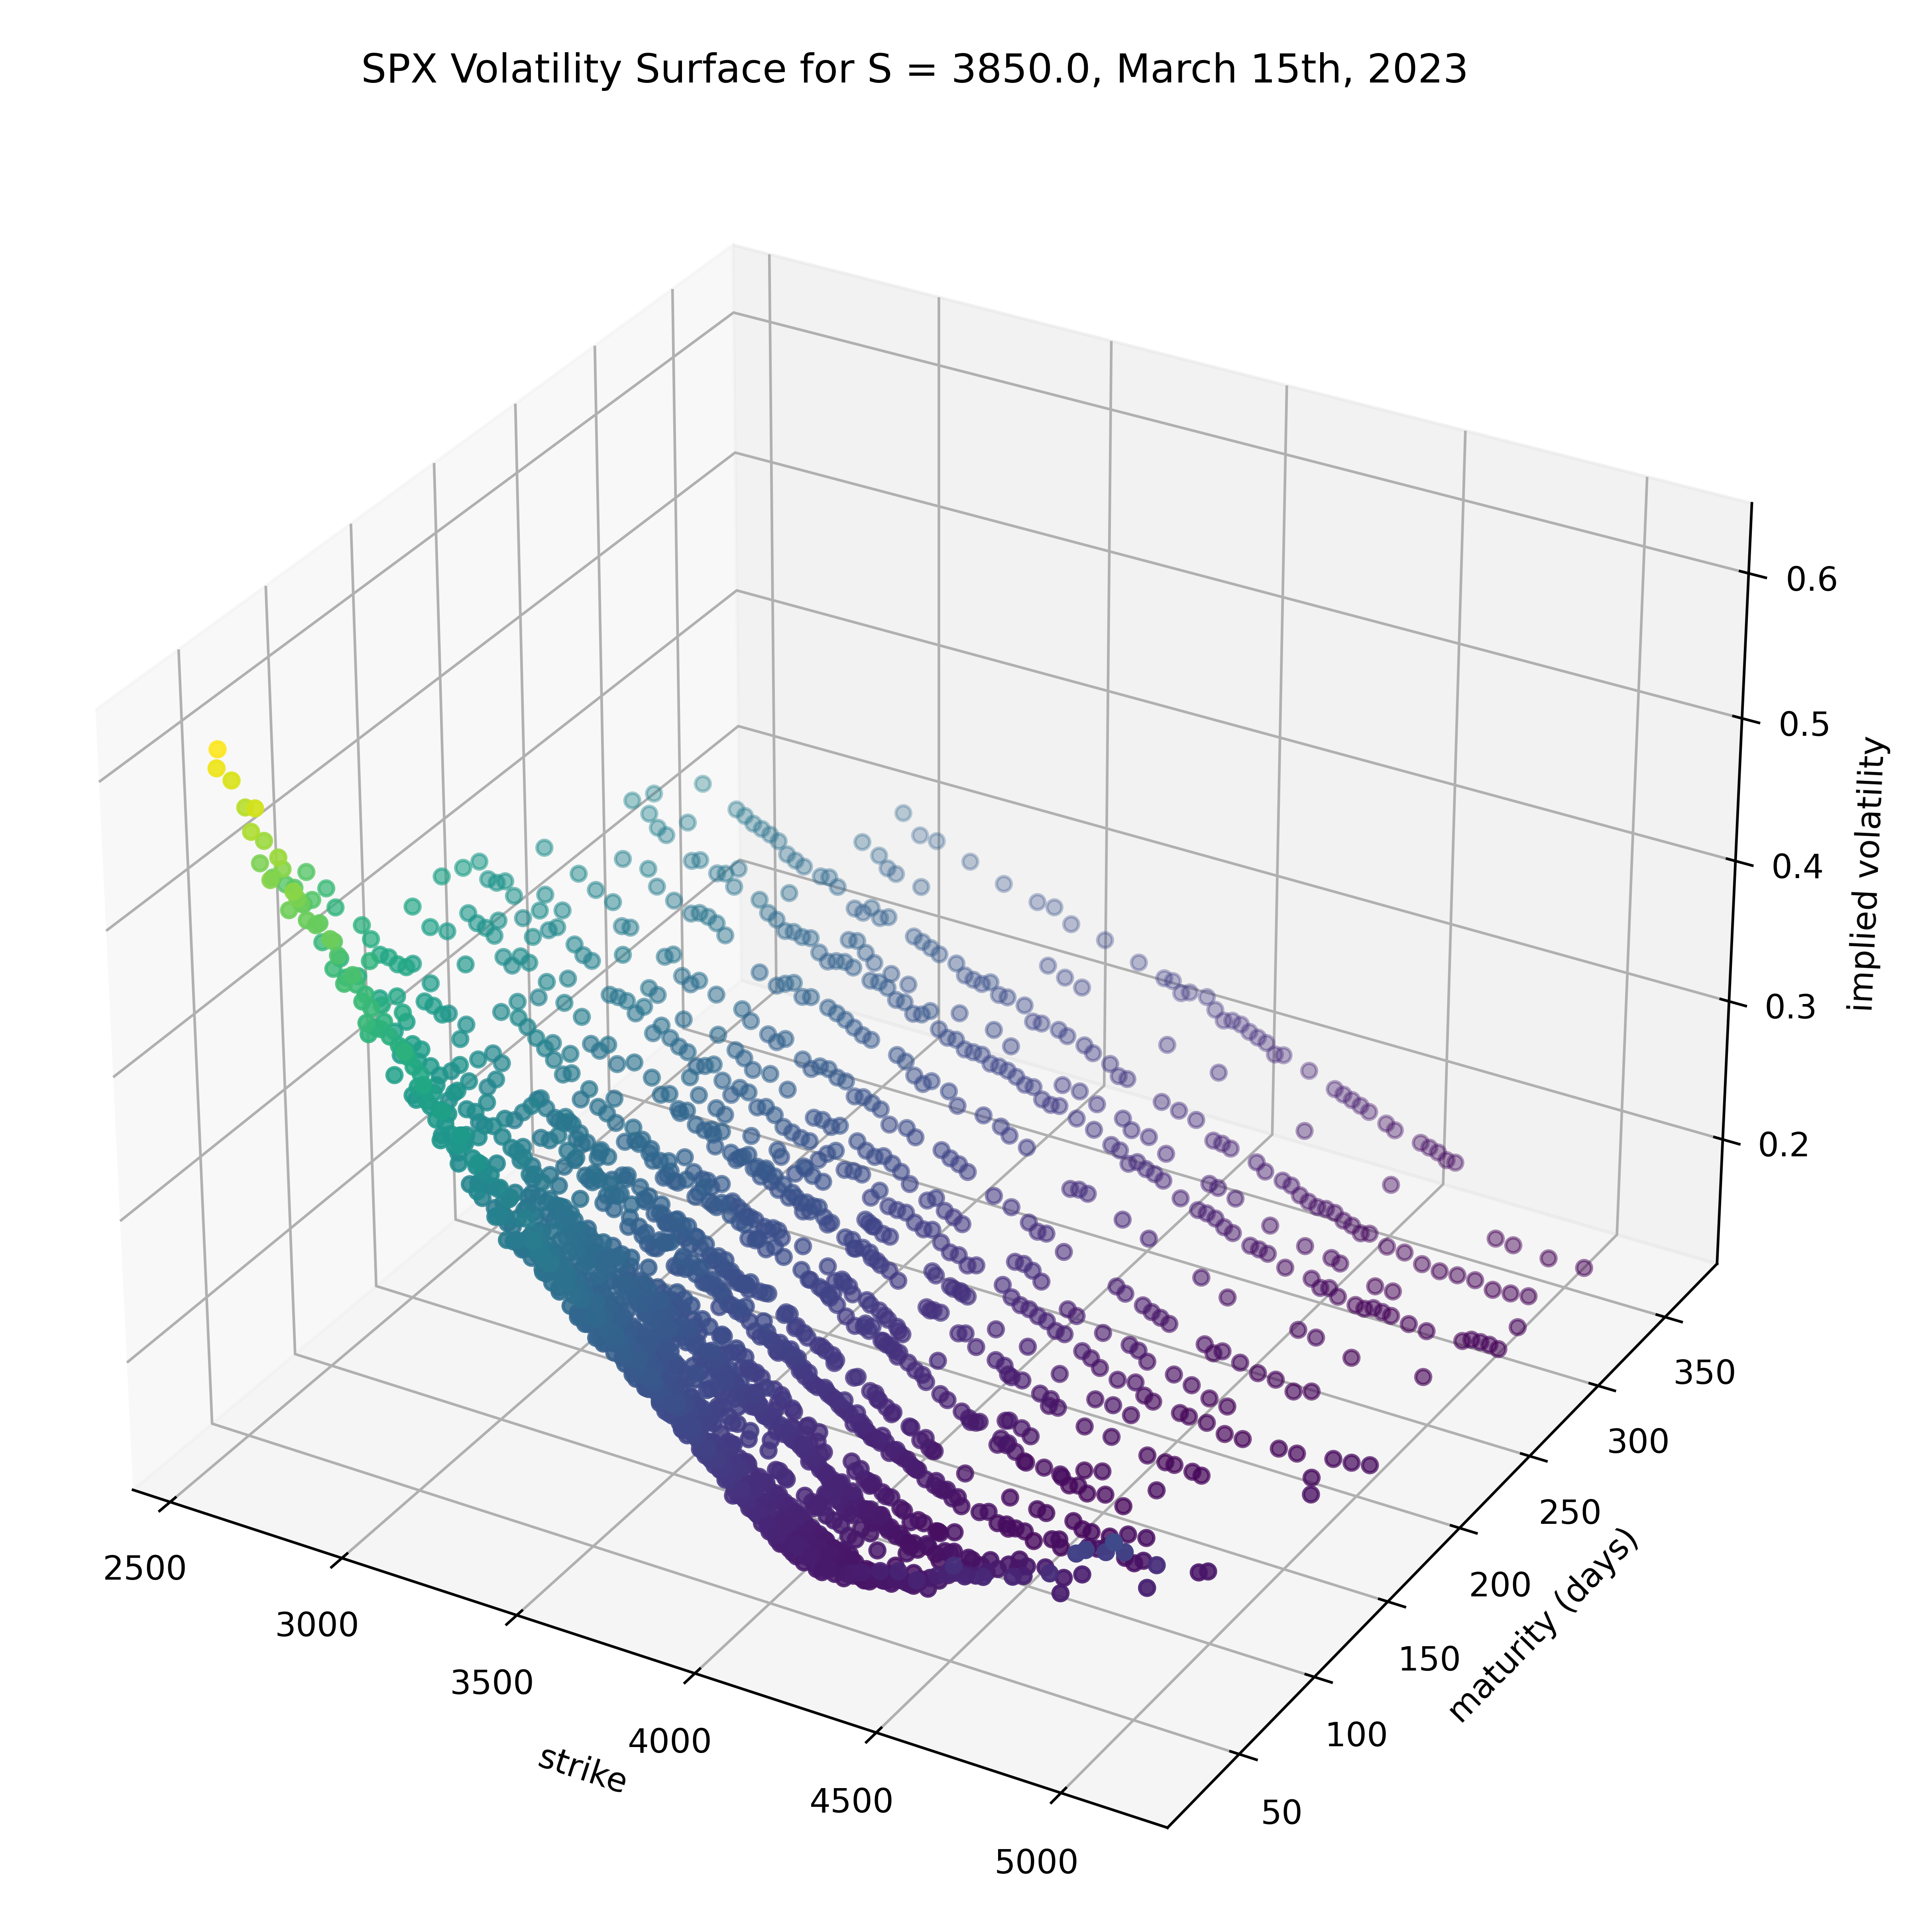
\includegraphics[width=\textwidth]{surface.png}
	\caption{Illustrative set of implied volatilities extracted from one day of SPX options trade data}
	\label{fig:surface}
\end{figure}
\newpage
\subsection{Distribution of market parameters}
\begin{figure}[h!]
	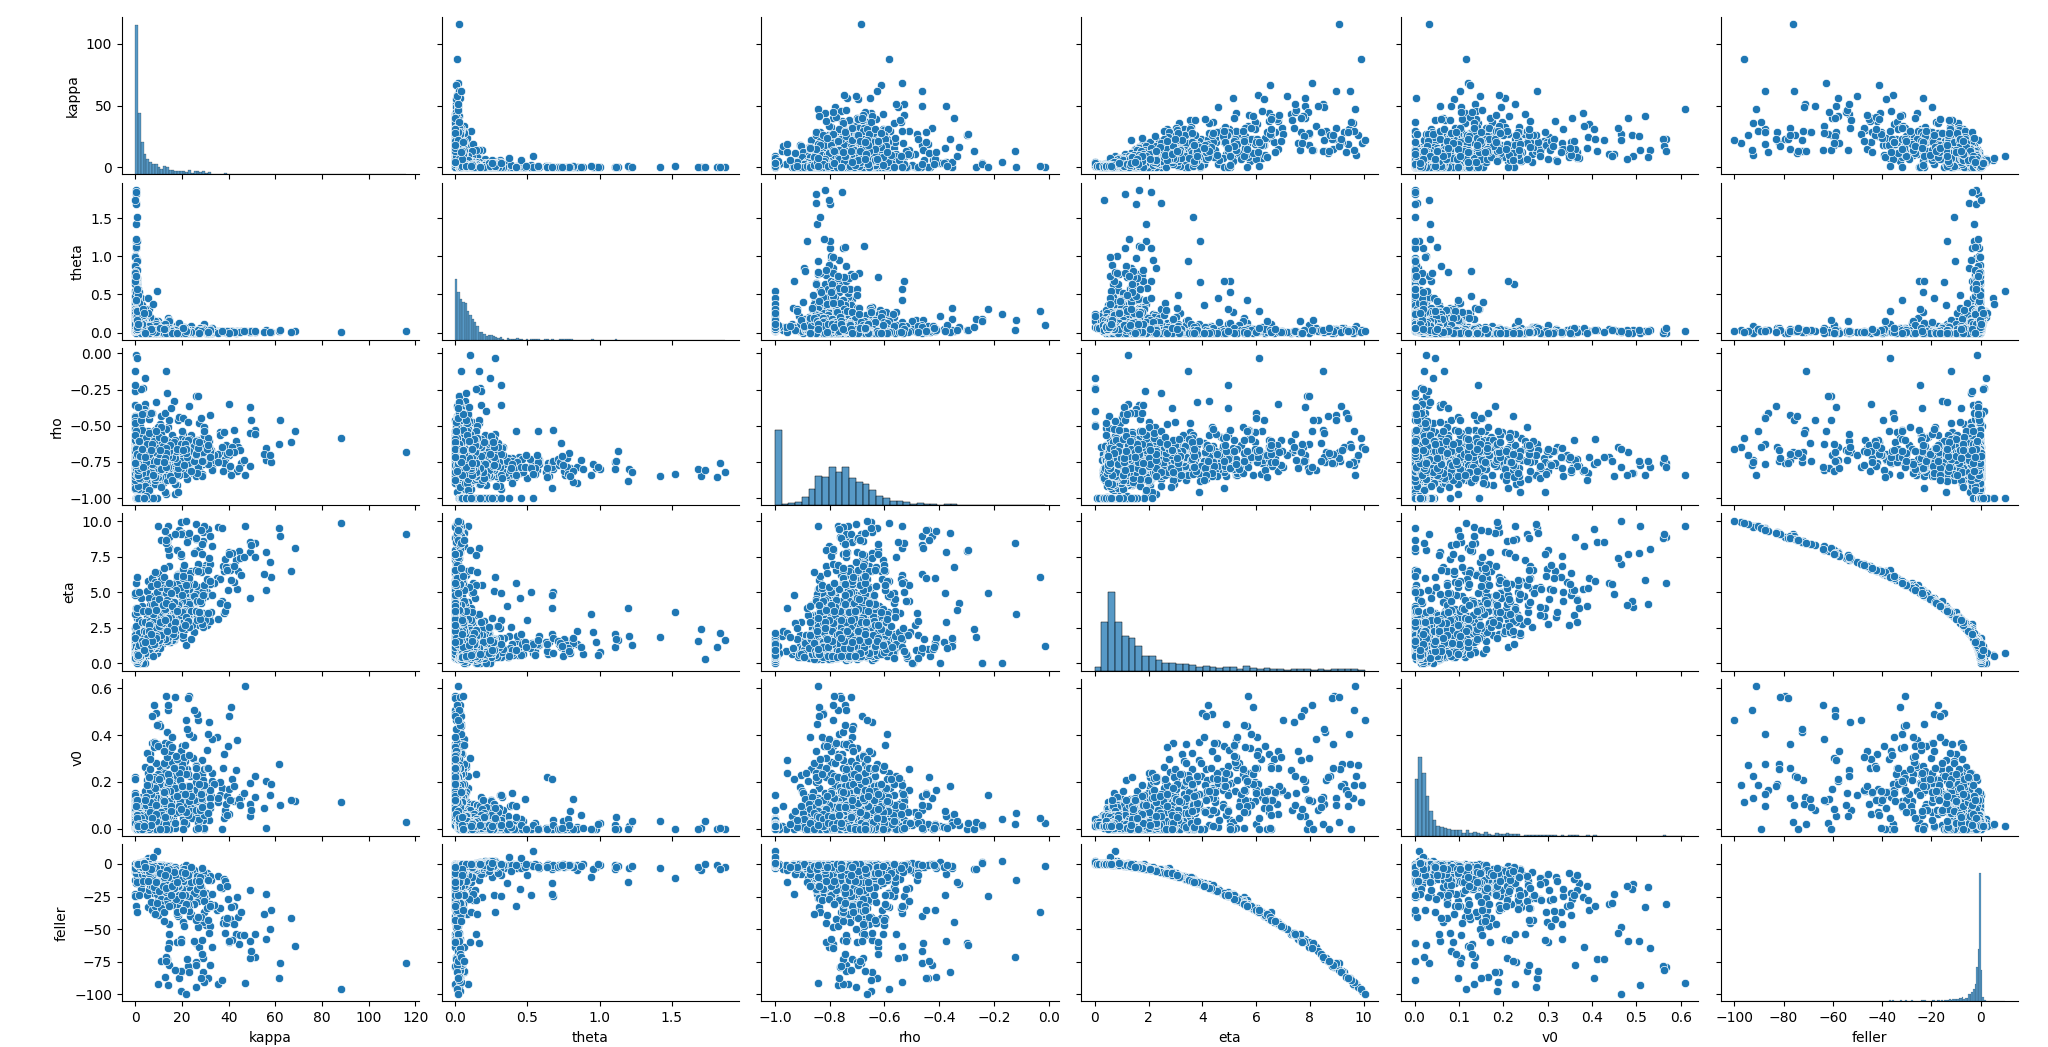
\includegraphics[width=0.98\textwidth]{market.png}
	\caption{Distribution of Heston~\cite{heston_1993_a} pricing model parameters}
	\label{fig:market}
\end{figure}
\end{document}